\cleardoublepage
\chapter{Introduction to standing waves and HIFI}
\label{sec:chapter1}



%#############################################################################
\section{The Heterodyne Instrument for the Far Infrared}
\sectionmark{Herschel/HIFI}

The Heterodyne Instrument for the Far Infrared (HIFI) on the Herschel Space Observatory is a heterodyne spectrometer that operates at frequencies between \SI{480}{\giga\hertz} and \SI{1910}{\giga\hertz},
producing spectra with a resolution ranging from \SI{1}{\mega\hertz} to \SI{125}{\kilo\hertz}~\cite{AA_518_L6}.
This high frequency resolution enables the astronomers to study the chemistry and dynamics of a wide range of phenomena, from planetary atmospheres to star forming regions.




%=============================================================================
\subsection{The Herschel Space Observatory}
\subsubsection{The satellite}
The Herschel Space Observatory (HSO) is named after Friedrich Wilhelm Herschel who discovered the existence of infrared radiation in 1800 (\cref{fig:herschel_discovers_infrared}).
The HSO was in operation from 2009 to 2013.
\begin{figure}[htbp]
    \centering
    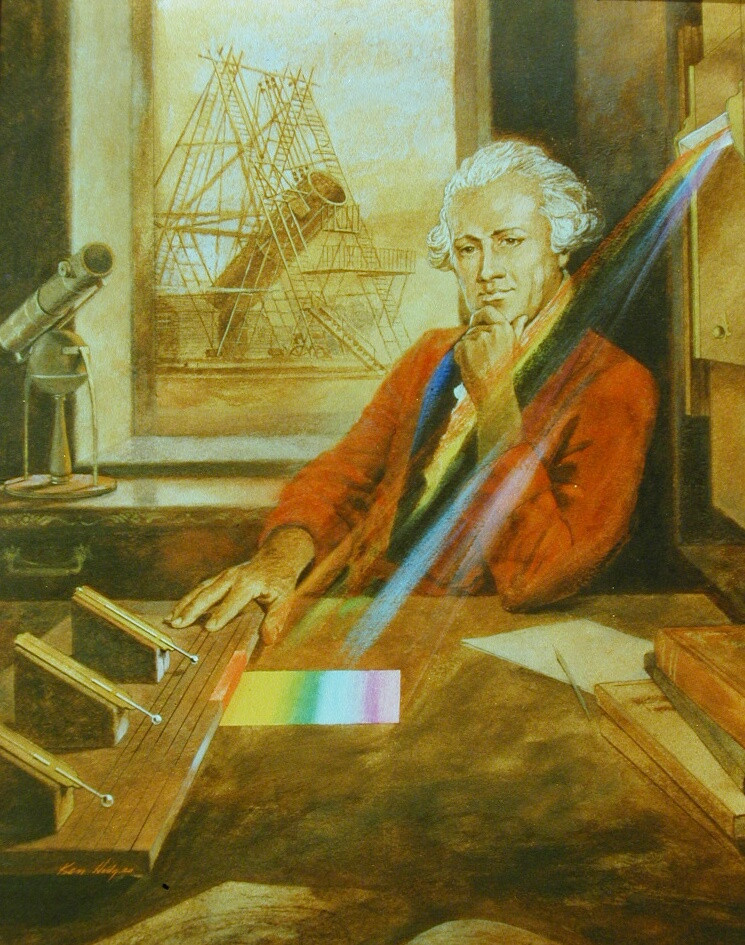
\includegraphics[height=8cm]{herschel_discovers_infrared}
    \caption{Herschel discovering infrared radiation.}
    \caption*{
        A prism decomposes the sunlight.
        The thermometer does not receive any visible sunlight but registers an elevation of temperature nonetheless:
        the sun emits an invisible radiation beyond the red color.
        Painting: Ken Hodges, 19\textsuperscript{th} century.
    }
    \label{fig:herschel_discovers_infrared}
\end{figure}

A significant fraction of the Universe consists of gas and dust that is too cold to radiate visible light.
This cold material is associated with the earliest stages of galaxy evolution, with star formation, protoplanetary disks and the atmosphere of comets.
With temperatures between ten and a few hundred Kelvin, the emission of these gases and dusts peaks in the far infrared.
Far infrared is the region of the electromagnetic spectrum between 0.3 and \SI{20}{\tera\hertz}.
In term of wavelength, the far infrared region ranges from \SI{15}{\micro\meter} to \SI{1}{\milli\meter}.
As shown on~\cref{fig:atmospheric_electromagnetic_opacity}, the Earth atmosphere is opaque to most of these wavelengths.
This is why observations in the far infrared are preferably done from space.

\begin{figure}[hbtp]
    \centering
    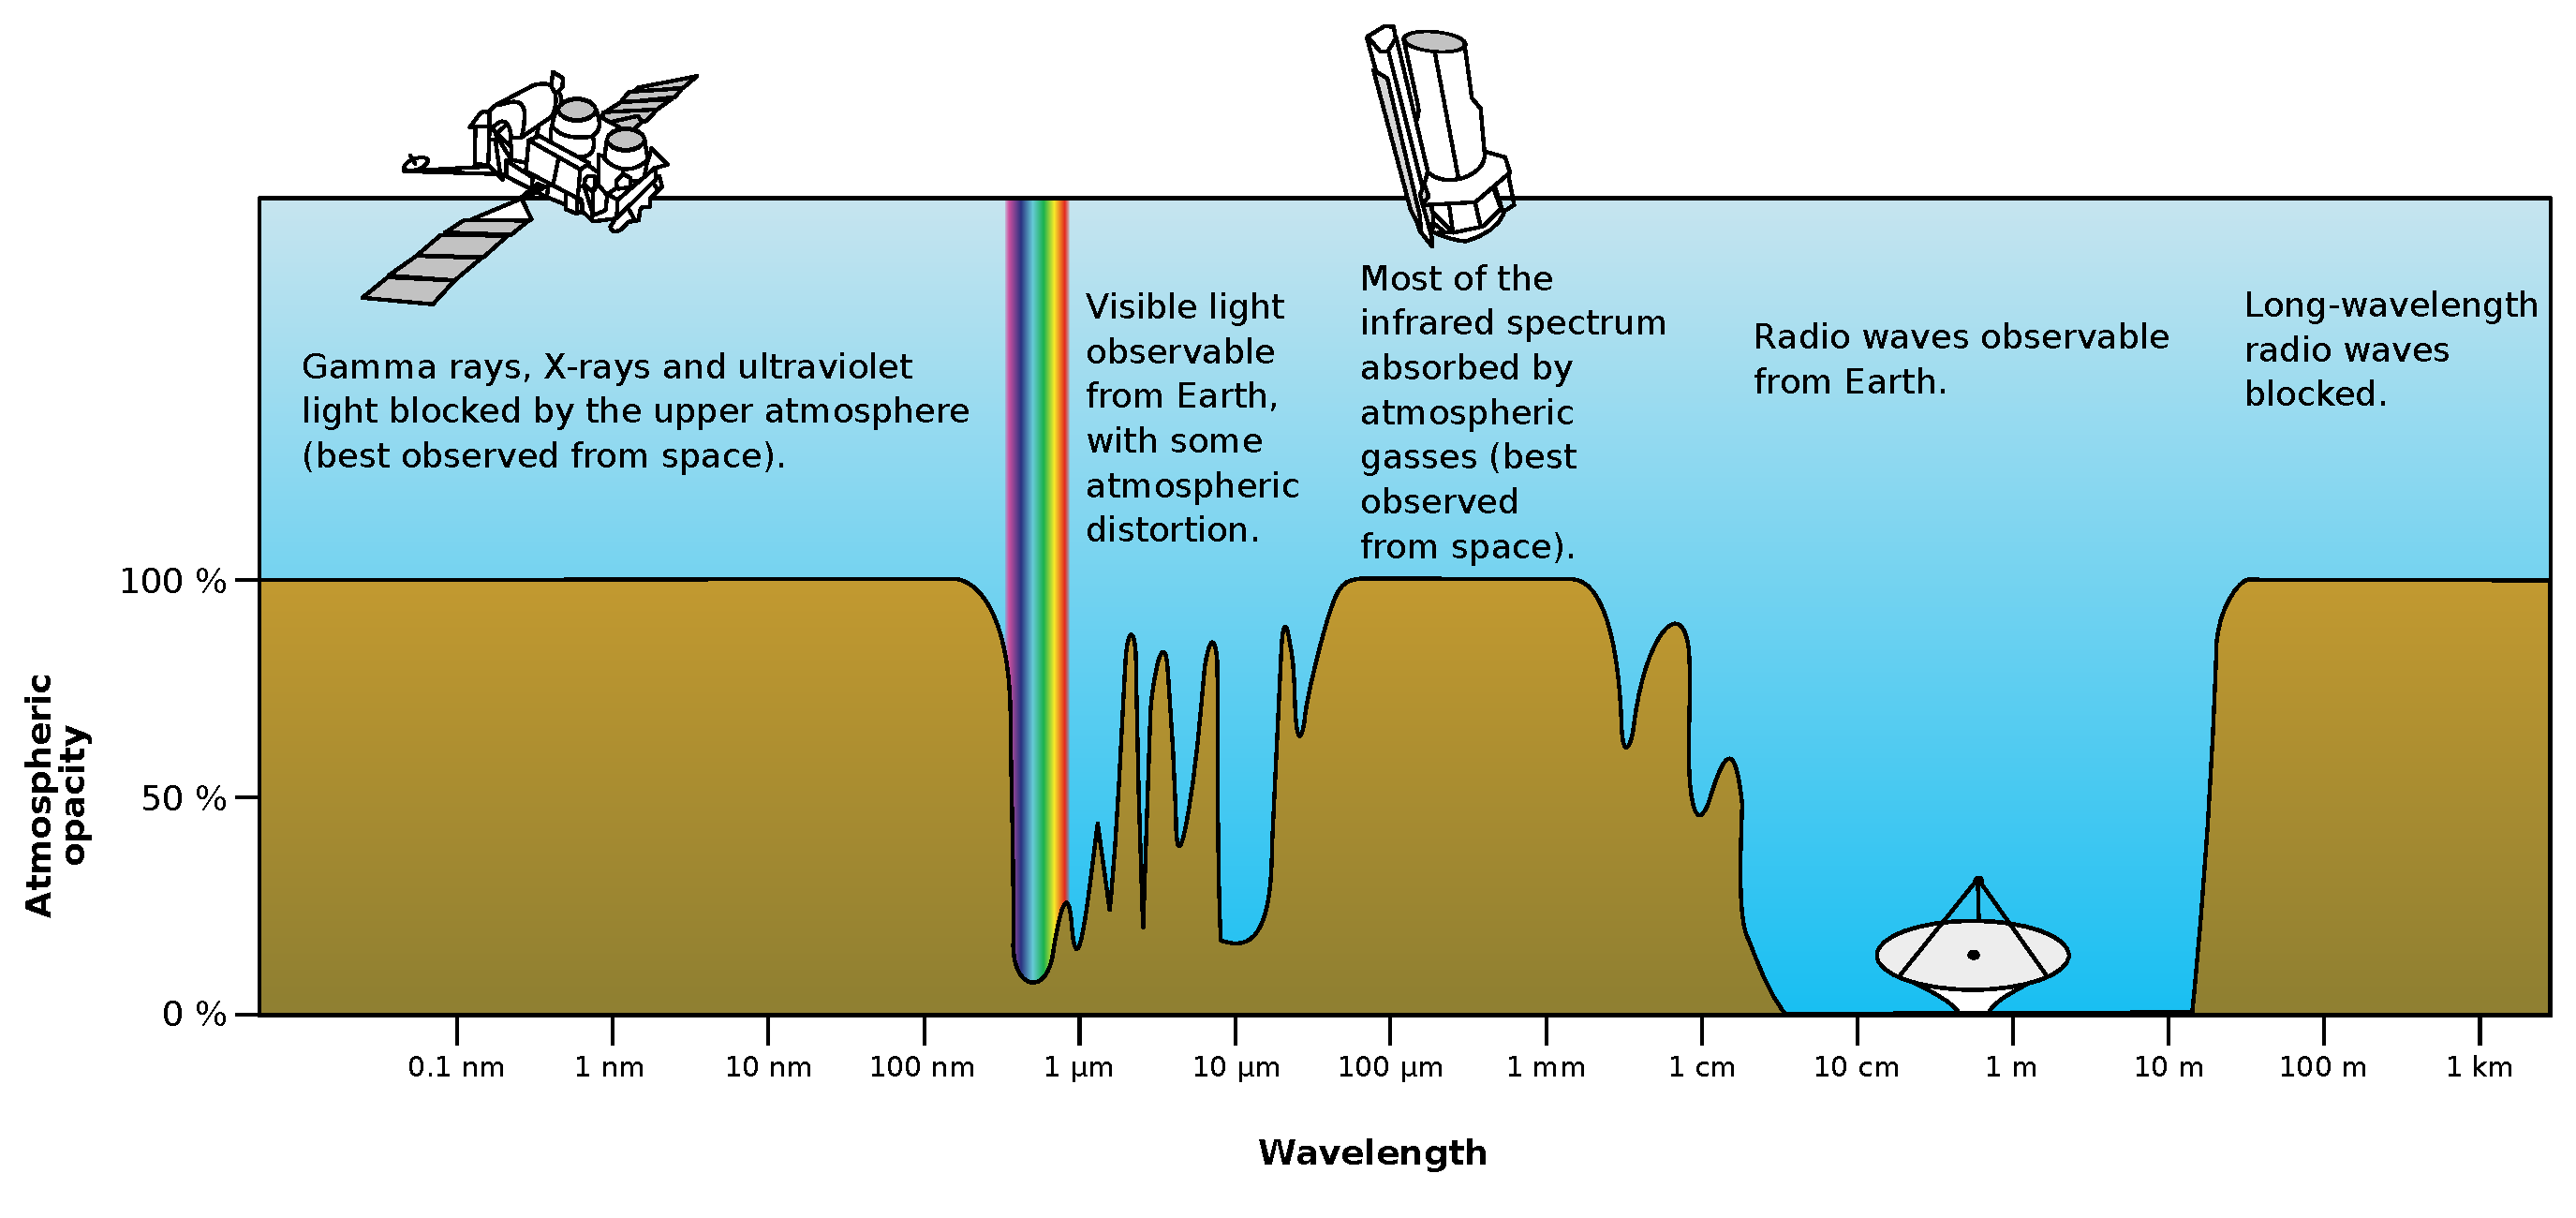
\includegraphics[width=\textwidth]{atmospheric_electromagnetic_opacity}
    \caption{Atmospheric electromagnetic opacity as a function of wavelength.}
    \caption*{Image: NASA.}
    \label{fig:atmospheric_electromagnetic_opacity}
\end{figure}

The HSO,
shown on~\cref{fig:herschel_spacecraft_artist},
was built and launched with the purpose of studying the cold Universe.
Its instrumentation covers wavelengths between 55 and \SI{672}{\micro\meter}.

\begin{figure}[hbtp]
    \centering
    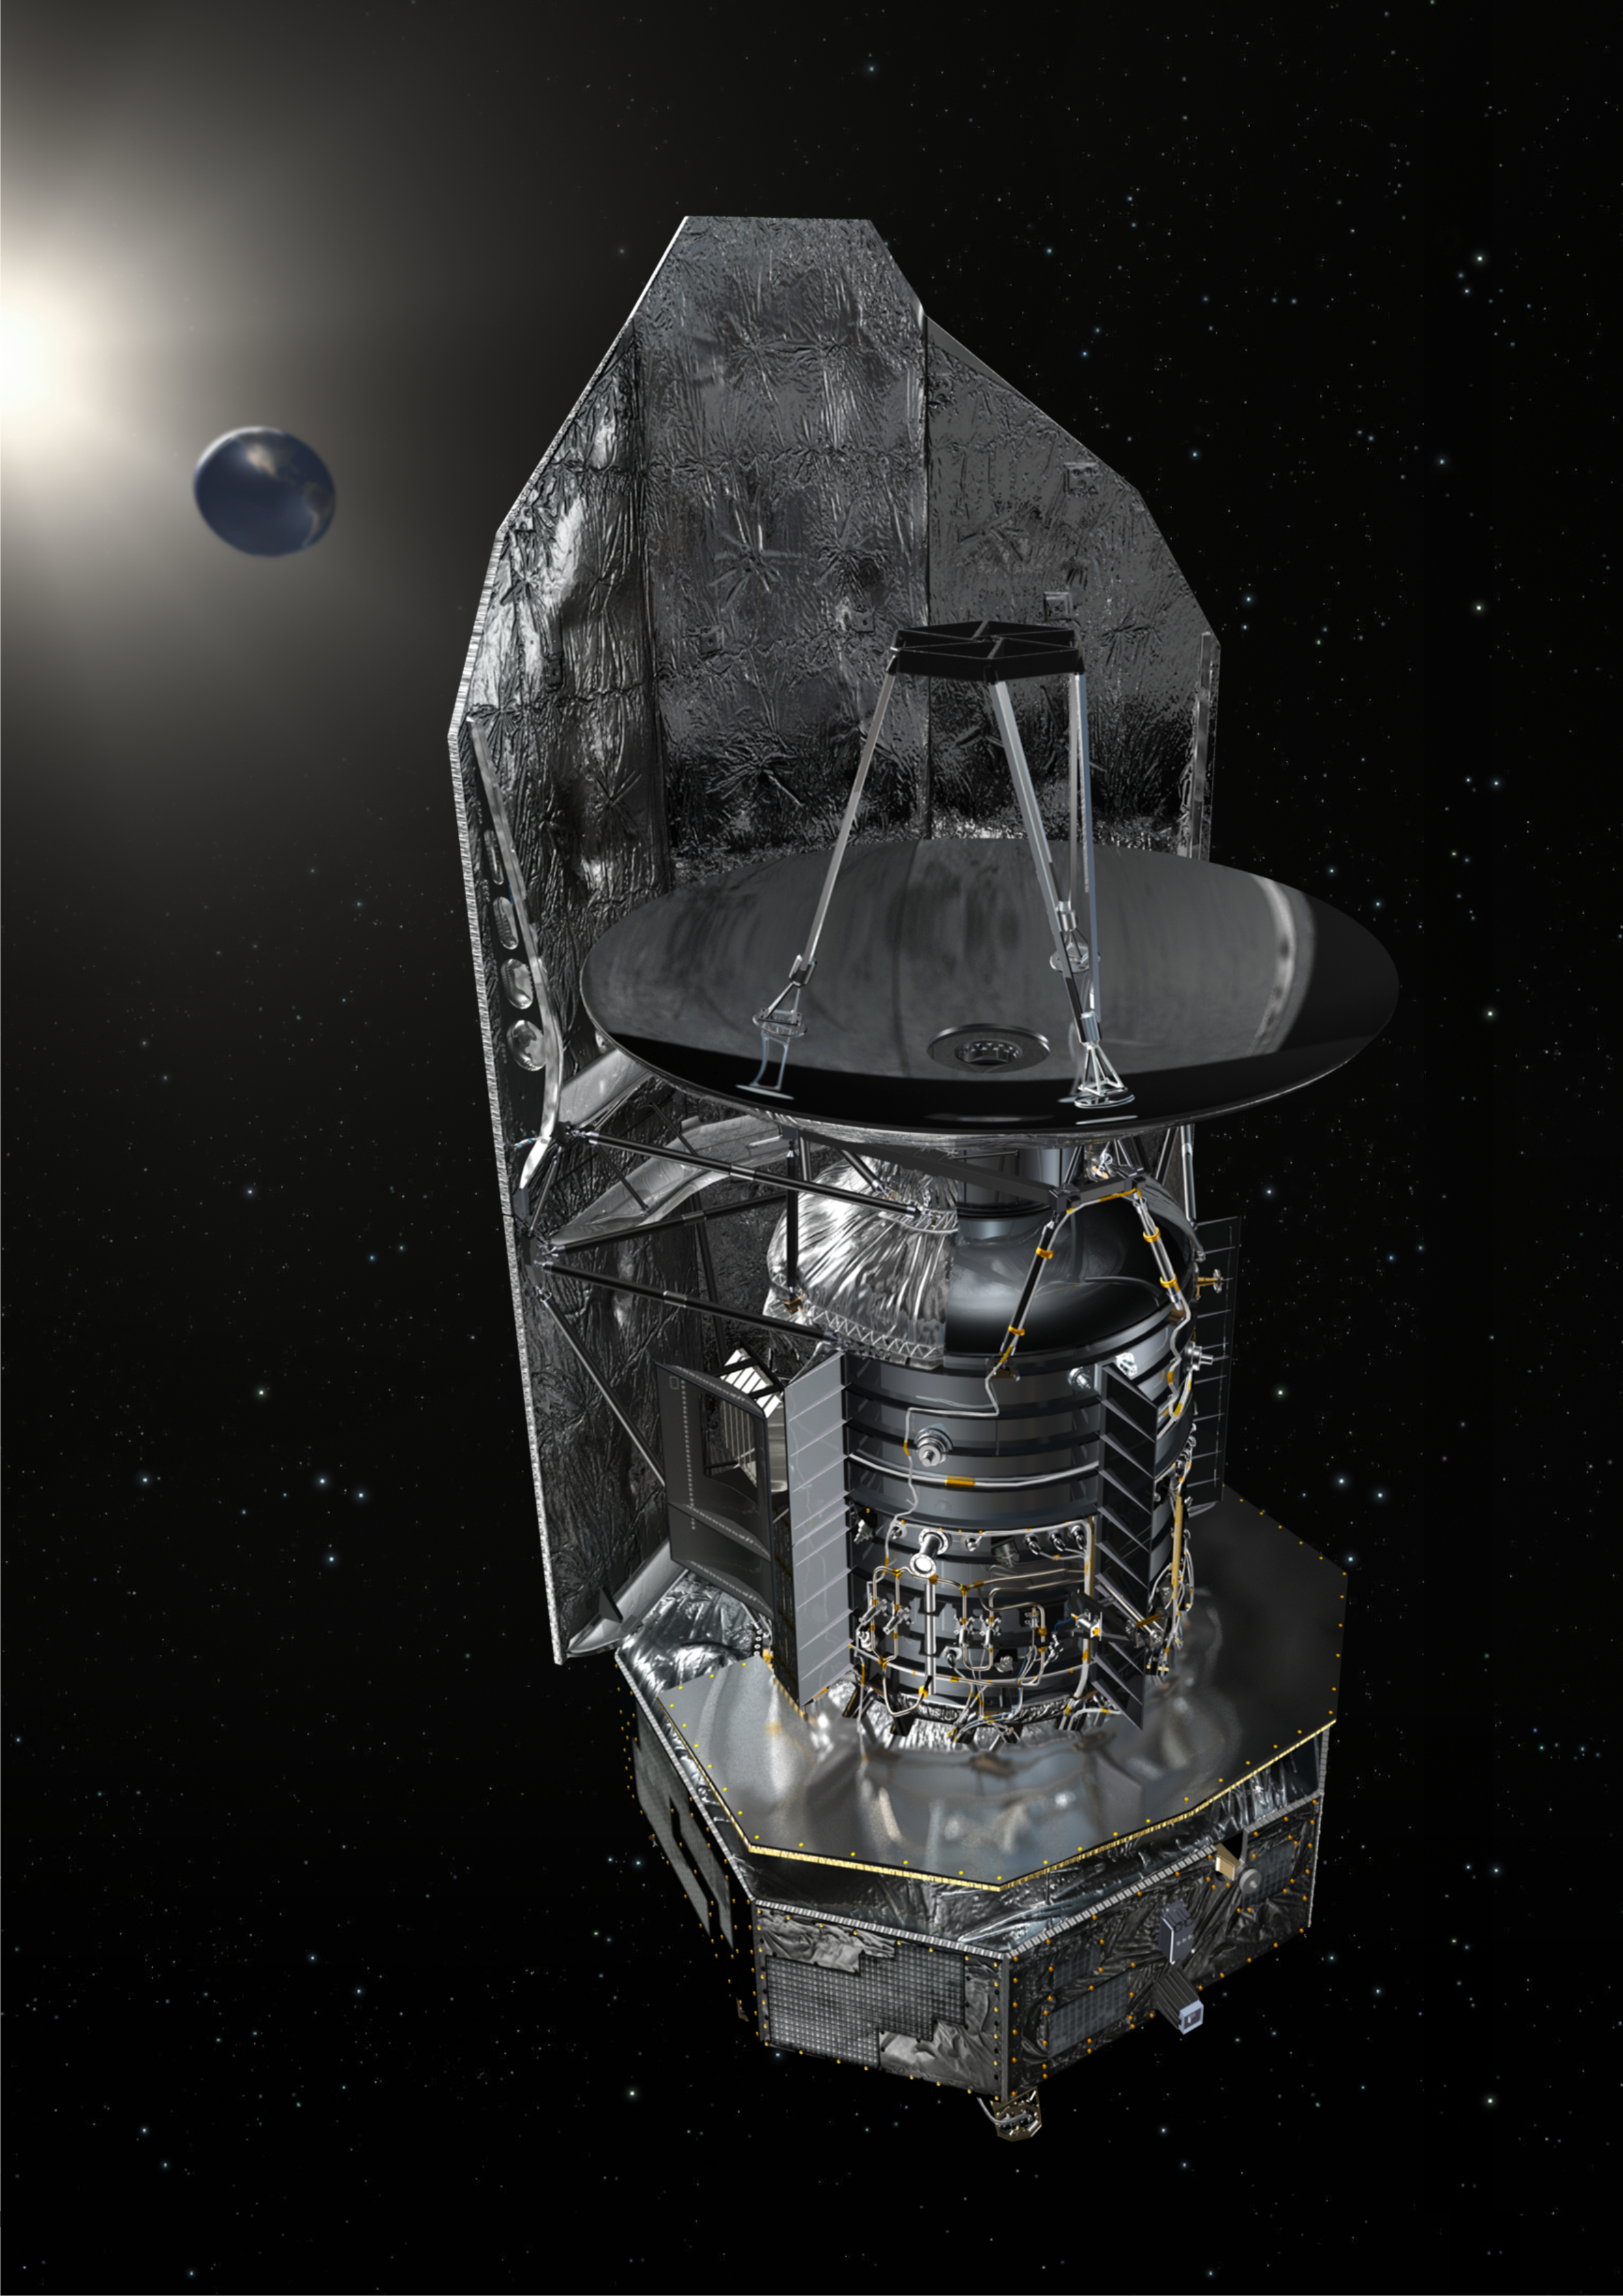
\includegraphics[height=8cm]{herschel_spacecraft_artist}
    \caption{Artist's impression of the Herschel Space Observatory.}
    \caption*{Image: ESA/AOES Medialab.}
    \label{fig:herschel_spacecraft_artist}
\end{figure}

During its operation, Herschel was orbiting the Lagrangian point $\text{L}_2$ of the Sun-Earth system, 1.5 million kilometers away from Earth (4~times the distance between Earth and the Moon).
The $\text{L}_2$ point lies on the line through the two large masses, beyond the smaller of the two (\cref{fig:herschel_spacecraft_artist}).
Here, the gravitational forces of the two large masses balance the centrifugal effect on a body at $\text{L}_2$.
The Sun-Earth $\text{L}_2$ is a good spot for space-based observatories.
Because an object around $\text{L}_2$ will maintain the same relative position with respect to the Sun and Earth, shielding and calibration are much simpler.
$\text{L}_2$ is too far away from Earth to be affected by its shadow;
this enables Herschel to use solar panels to convert sunlight into energy,
but it also warms up the satellite.

Observing the cold Universe with a warm telescope is like observing faint stars in broad day daylight.
To prevent that, the instruments of Herschel are cooled down in a superfluid helium cryostat\index{cryostat} (\cref{fig:photo_hifi_cryo}).
The cryostat provides temperature between~\SI{1.7}{\kelvin} at its coolest point, up to \SI{10}{\kelvin} where lower temperatures are not required.
The primary mirror itself is not actively cooled down but is shielded from direct sunlight by a sun shade; it has a temperature of approximately~\SI{70}{\kelvin}.

With \SI{2300}{\liter} of Helium on board slowly boiling off at \SI{1.4}{\kelvin}, the mission had a predicted life time of 3.5~years.
Herschel exceeded that requirement by remaining in operation 3.96~years.
Herschel was deorbited from $\text{L}_2$ on the 29\textsuperscript{th} of April 2013 and is now parked on a solar orbit, all its electronics (including communication) shut down, where it will not encounter Earth for hundreds of years.

\begin{figure}[hbtp]
    \centering
    \includegraphics[width=.8\textwidth]{herschel_s_cryostat_vacuum_vessel}
    \caption{Herschel's cryostat vacuum vessel.}
    \caption*{The Herschel cryostat vacuum vessel, seen here in the ESTEC cleanroom, stores 2370 liters of superfluid liquid helium (He II) which is used to help cool the various elements of the detector plane. In orbit, the black outer half of the vessel faces away from the Sun and acts as a radiator while the reflective half faces the inside of the sunshade and reflects excess heat.  Photo: ESA, 2007.}
    \label{fig:photo_hifi_cryo}
\end{figure}

Herschel's primary mirror\index{mirror, primary} has a diameter of~\SI{3.5}{\meter}, which makes Herschel the widest telescope ever launched in space at the time of writing (2014).
With a mass of~\SI{3300}{\kilo\gram}, it is also the heaviest.
\Cref{fig:photo_herschel} shows a photograph of the HSO at the European Space Research and Technology Center (ESTEC), with engineers for scale.
In comparison, the Hubble Space Telescope has a diameter of~\SI{2.4}{\meter} but is optical.
In infrared, the other telescopes are the Infrared Space Observatory\index{ISO} (ISO)~\cite{isoHandbook1} with~\SI{60}{\centi\meter} and Spitzer\index{Spitzer} with~\SI{85}{\centi\meter}.
The diameter of Herschel gives it a sensitivity and a spatial resolution that had never been achieved at these wavelengths.
That diameter was limited only by the size of the fairing of the Ariane 5 rocket which launched it from Kourou, French Guiana, on the 14\textsuperscript{th} of May 2009 (\cref{fig:ariane_5_lift_off}).
Thanks to a modular design, The James Webb Space Telescope\index{JWST} (JWST), planned to be launched in 2018, will have a~\SI{6.5}{\meter} primary mirror but will focus on the near infrared.

\begin{figure}[hbtp]
    \centering
    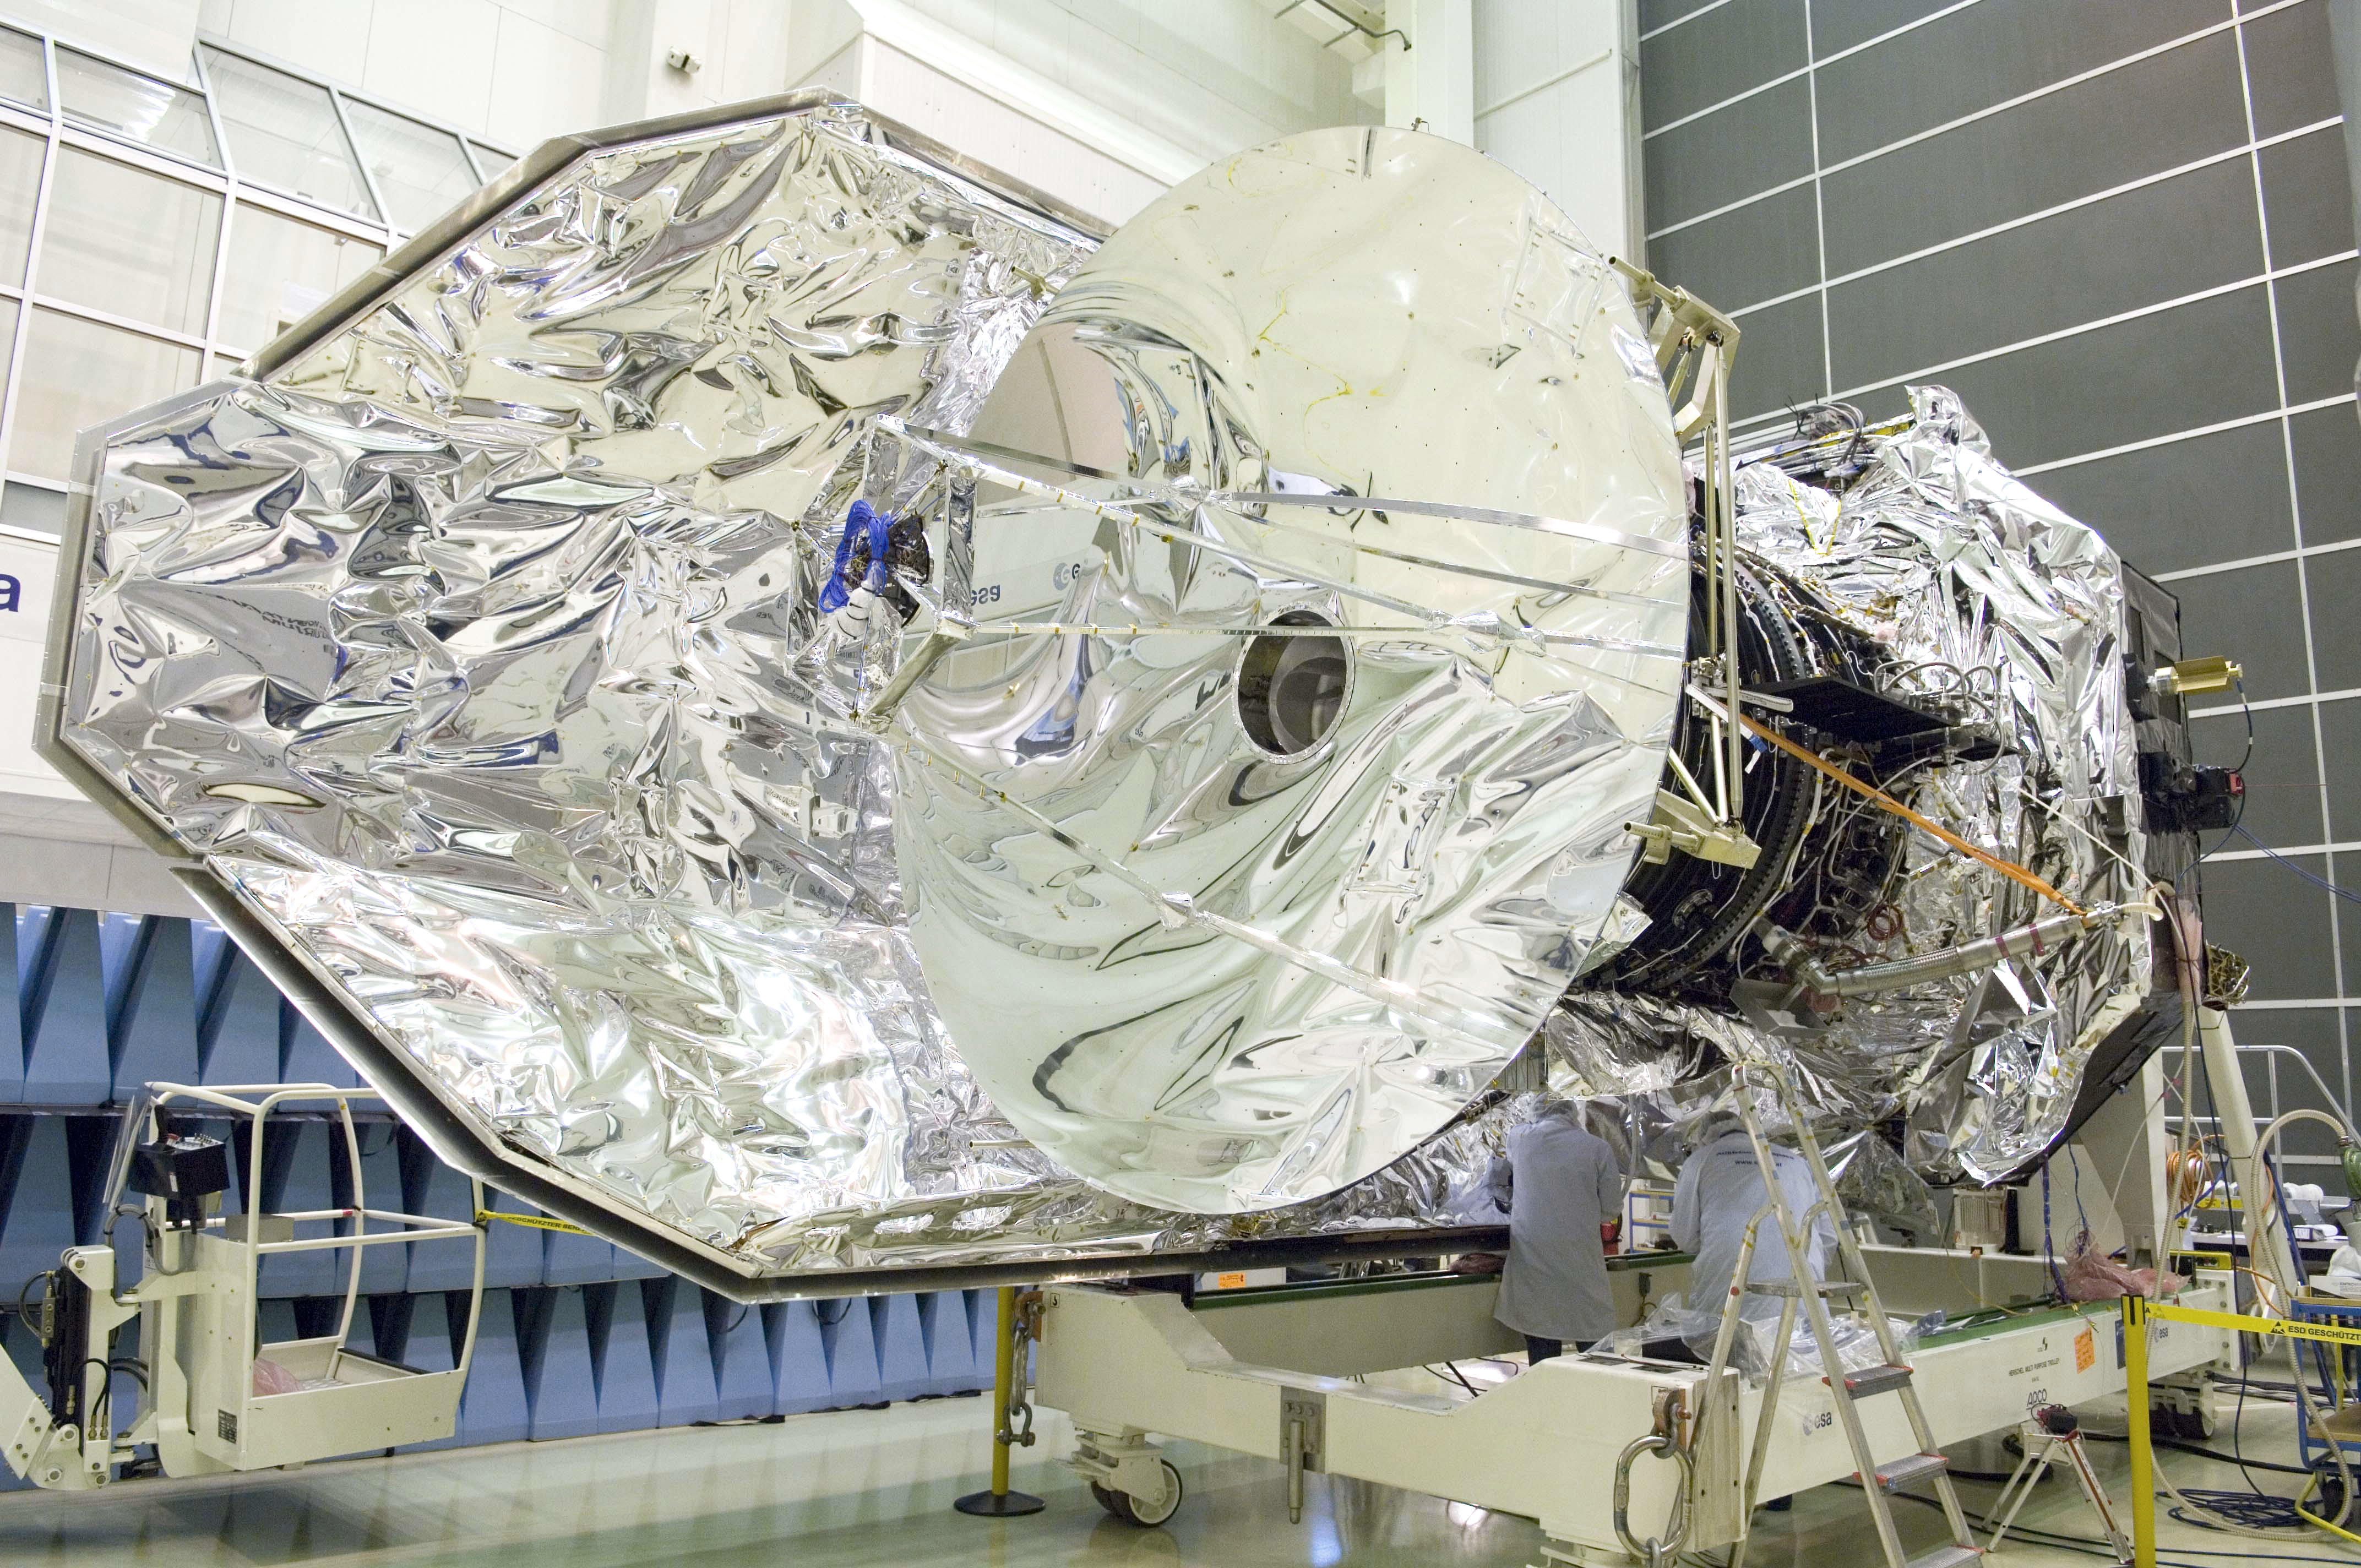
\includegraphics[width=.8\textwidth]{herschel_spacecraft}
    \caption{The Herschel spacecraft.}
    \caption*{The flight model of the Herschel spacecraft mounted on its multipurpose trolley in a horizontal position for the the high-precision measurements of the distance between its primary and secondary mirrors (M1 and M2).  Photo: ESA, 2009.}
    \label{fig:photo_herschel}
\end{figure}

\begin{figure}[hbtp]
    \centering
    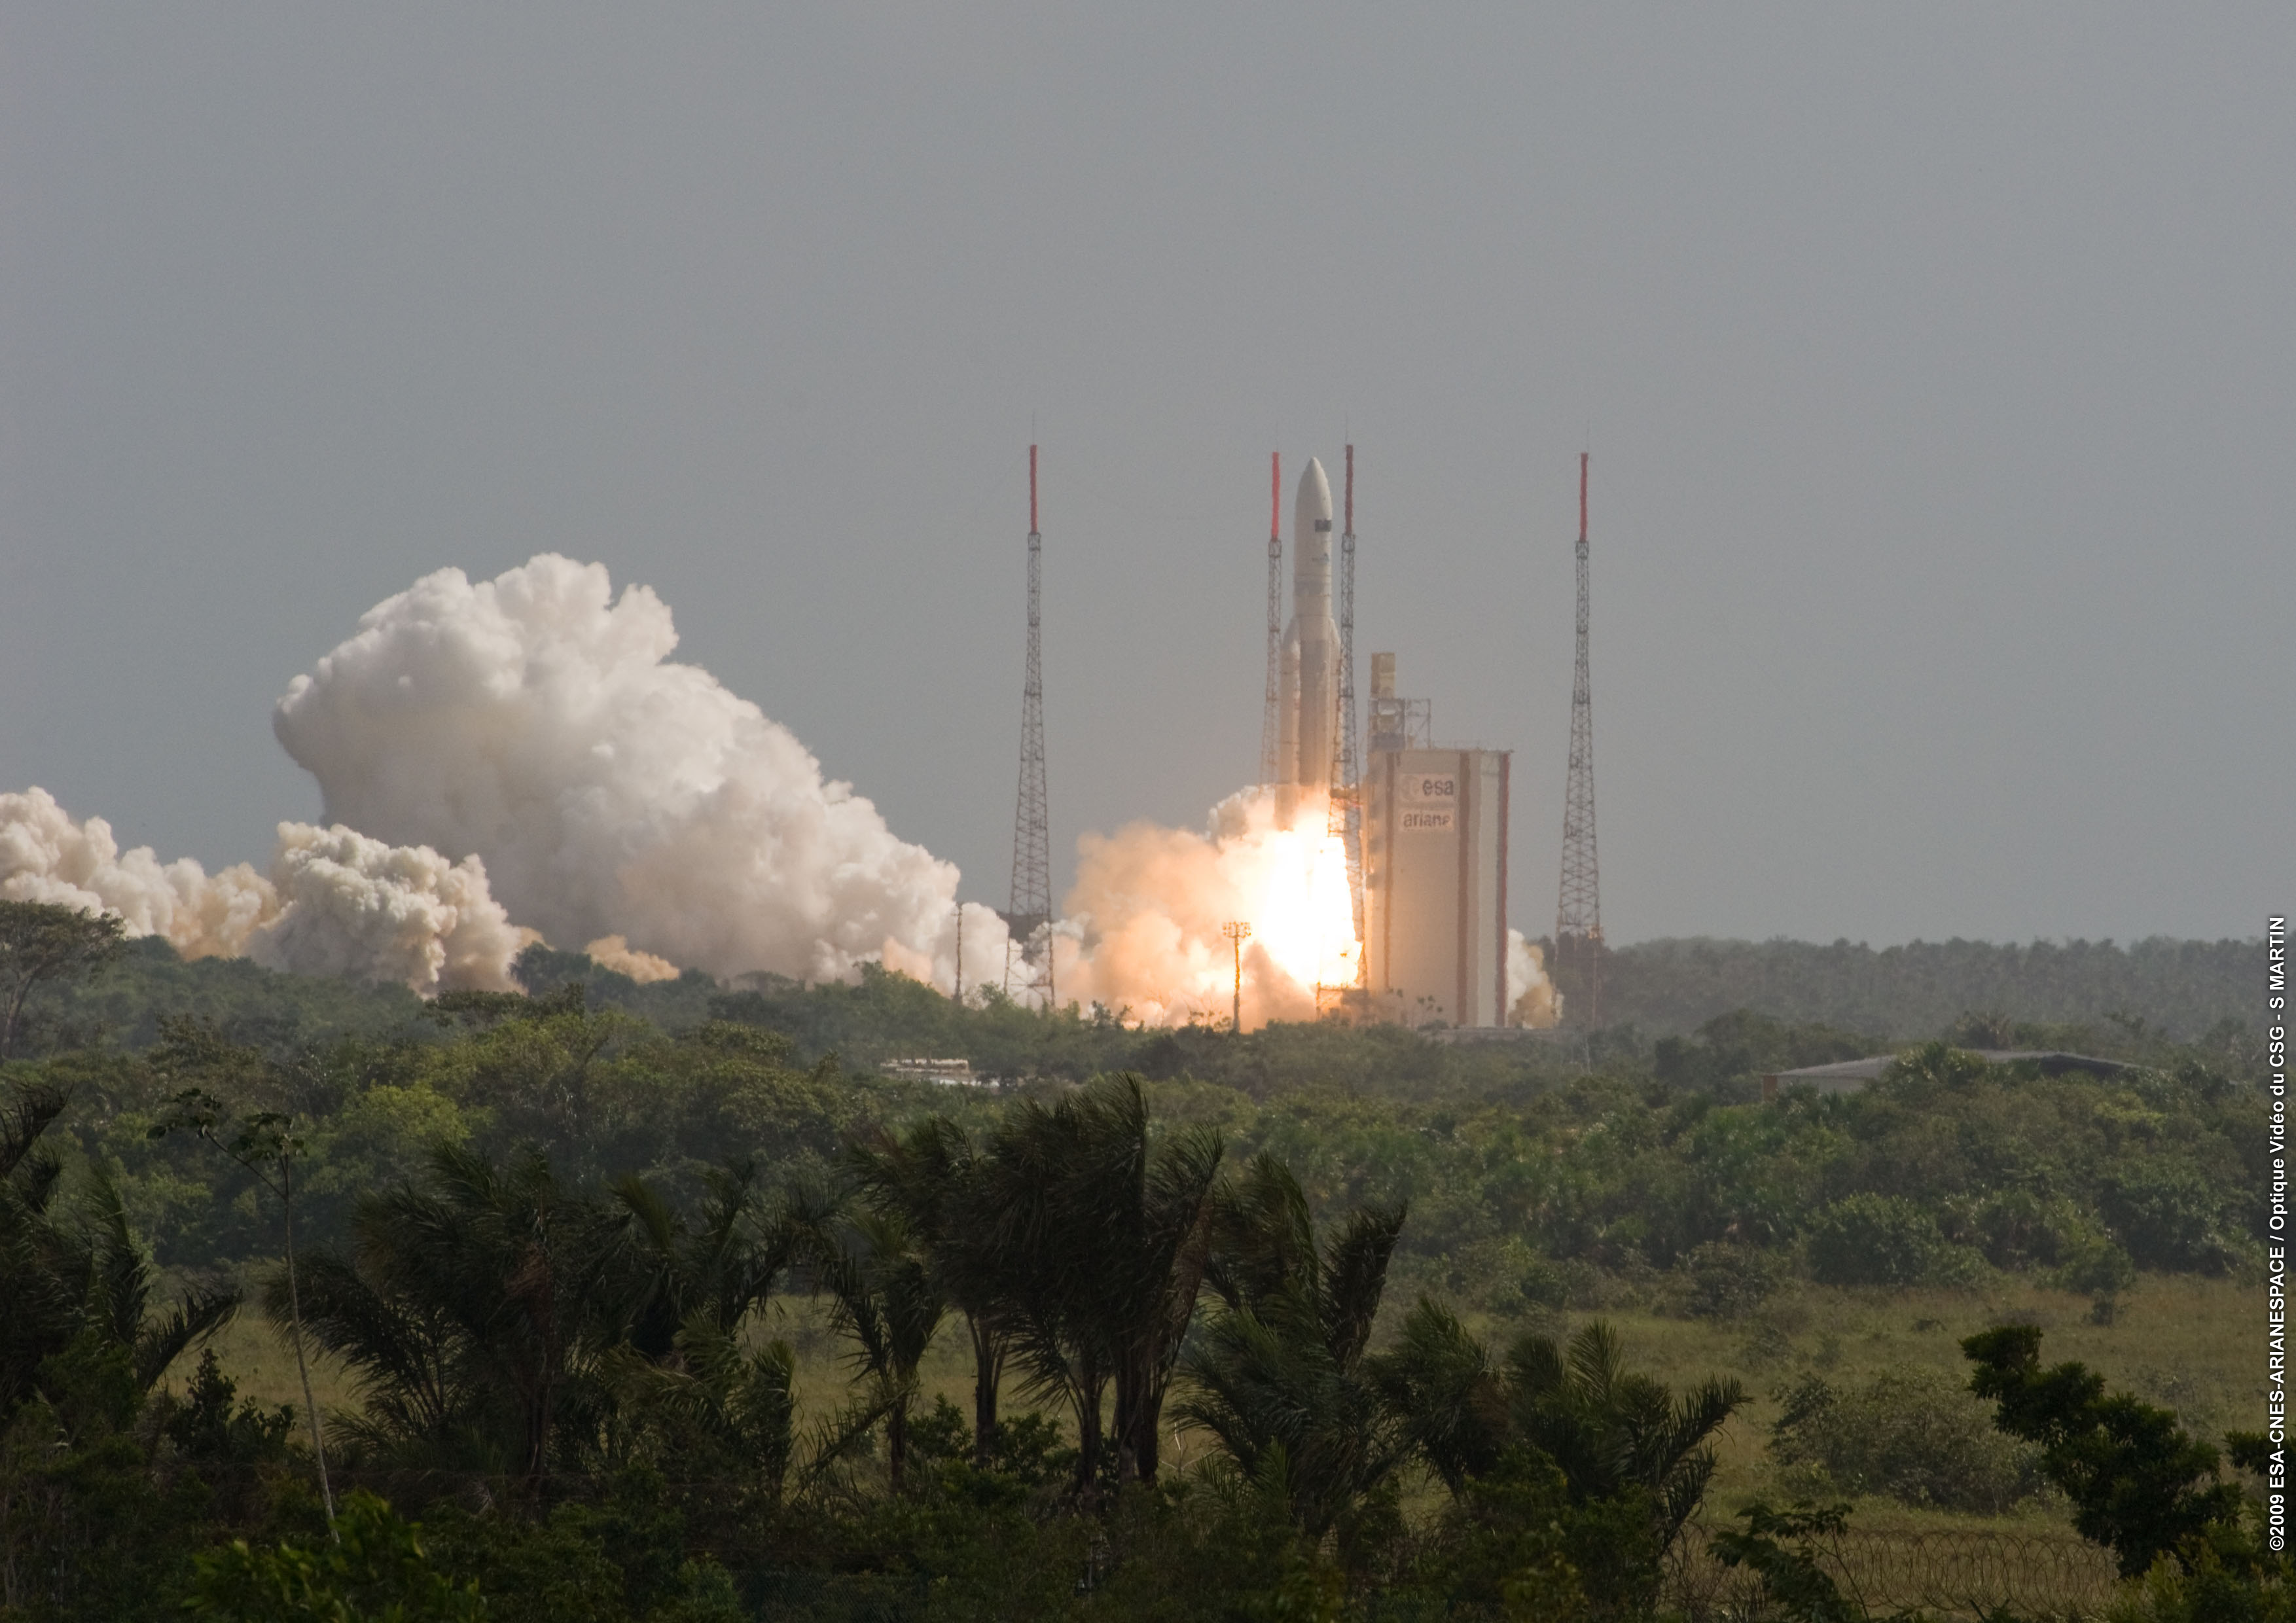
\includegraphics[width=.8\textwidth]{ariane_5_lift_off}
    \caption{Ariane 5 lift off.}
    \caption*{
        At 15:12:02 CEST on 14 May 2009,
        at the beginning of a 55-minute launch window,
        the Herschel and Planck satellite pair lifted off on board an Ariane 5 from Europe's Spaceport in French Guiana.
    Photo: ESA/CNES/ARIANESPACE - Photo Optique Video CSG, P. Baudon, 2009.}
    \label{fig:ariane_5_lift_off}
\end{figure}

The European Space Agency\index{ESA} (ESA) built and operated Herschel.
The National Aeronautics and Space Administration\index{NASA} (NASA) brought a significant contribution to the project.
The Common Service Module was designed and built by Thales Alenia Space\index{Thales Alenia Space}.

The reader interested in a more detailed description of Herschel is invited to read \citetitle{AA_518_L1} by \citeauthor{AA_518_L1}~\cite{AA_518_L1}.

%-----------------------------------------------------------------------------
\subsubsection{The payload}

Herschel has three scientific instruments: PACS, SPIRE and HIFI.
Only one can be used at a time.

\paragraph{PACS.}\index{PACS}The Photodetecting Array Camera and Spectrometer%
~\cite{poglitsch2010photodetector}
comprises two mutually exclusive sub-instruments: a bolometric camera to perform photometry in three spectral bands (\num{70}, \num{100} and \SI{160}{\micro\meter}) and an integral field unit grating spectrometer operating over the spectral range from~\num{57} to~\SI{210}{\micro\meter} with a spectral resolution ranging from~\num{1000} to~\num{5000}.

The spectrometer of PACS provides information on the abundances of molecules
(\ce{CO}, \ce{H2O}, \ce{OH}) atomic species (\ce{O+}, \ce{O^2+}, \ce{C+}) and continuum.
This can be used for instance to determine which of these spectral lines are efficient at cooling the gas in star forming regions~\cite{2013A&A...552A.141K}.

The camera of PACS shone light on the ubiquity of the filamentary structure of star forming regions~\cite{2010A&A...518L.100M}.



\paragraph{SPIRE.}\index{SPIRE}The Spectral and Photometric Imaging Receiver%
~\cite{griffin2010herschel}
is also an imaging camera and a low-resolution spectrometer.
The camera has three bands centered at \num{250}, \num{350} and~\SI{500}{\micro\meter}.
The spectrometer has a resolution between \num{40} and~\num{1000} at~\SI{250}{\micro\meter}.

\todo[inline]{Science done with SPIRE?}

\paragraph{HIFI.}\index{HIFI}The Heterodyne Instrument for the Far Infrared%
~\cite{AA_537_A17}
is a high-resolution spectrometer.
It operates between~\num{157} and~\SI{650}{\micro\meter} and its spectral resolution can reach~$10^7$.
HIFI is a single-pixel instrument.

This book focuses on HIFI.
We will describe this instrument more thoroughly in~\cref{sec:HIFI}.



%=============================================================================
\subsection{HIFI}
\label{sec:HIFI}

The Heterodyne Instrument for the Far Infrared (HIFI) has a property that sets it apart from the other instruments of the Herschel Space Observatory: it is a coherent detector, in the electromagnetic sense of the term.
We will define the term ``coherence'' later,
in~\cref{sec:hifi_is_coherent}
on~\cpageref{sec:hifi_is_coherent}.
While this book explores the consequences of coherence on the calibration of detectors in general, we use HIFI as a practical example throughout its chapters.
We are now going to introduce HIFI in some details.


%-----------------------------------------------------------------------------

\subsubsection{A high-resolution spectrometer}

HIFI is a high-resolution spectrometer: its typical spectral resolution $R$ is~$10^6$.
Spectral resolution is defined as the ratio of two quantities: the frequency $f$ at which the instrument operates, and the bandwidth $\Delta f$ of its spectral channels; see~\cref{eq:spectral_resolution}.
\begin{equation}
    R = \frac{f}{\Delta f} \label{eq:spectral_resolution}
\end{equation}
For example, observing with the Wideband Spectrometer backend (WBS) of HIFI at~\SI{500}{\giga\hertz} yields a spectral resolution $R=\num{500000}$.
Indeed, in that example, $f=\SI{500e9}{\hertz}$ and $\Delta f=\SI{1e6}{\hertz}$.
This is a worst-case scenario for HIFI: using the less accurate backend near the lowest possible frequency.
The best case scenario would be to use the High-Resolution Spectrometer (HRS) backend at~\SI{1900}{\giga\hertz}:
$R=\num{15.2e6}$
with $f=\SI{1900e9}{\hertz}$
and $\Delta f=\SI{125e3}{\hertz}$.
In comparison with the spectral resolutions of the PACS and SPIRE instruments (between~\num{50} and~\SI{5000}), that of HIFI is at least three orders of magnitude better.

\begin{figure}[hbtp]
    \centering
    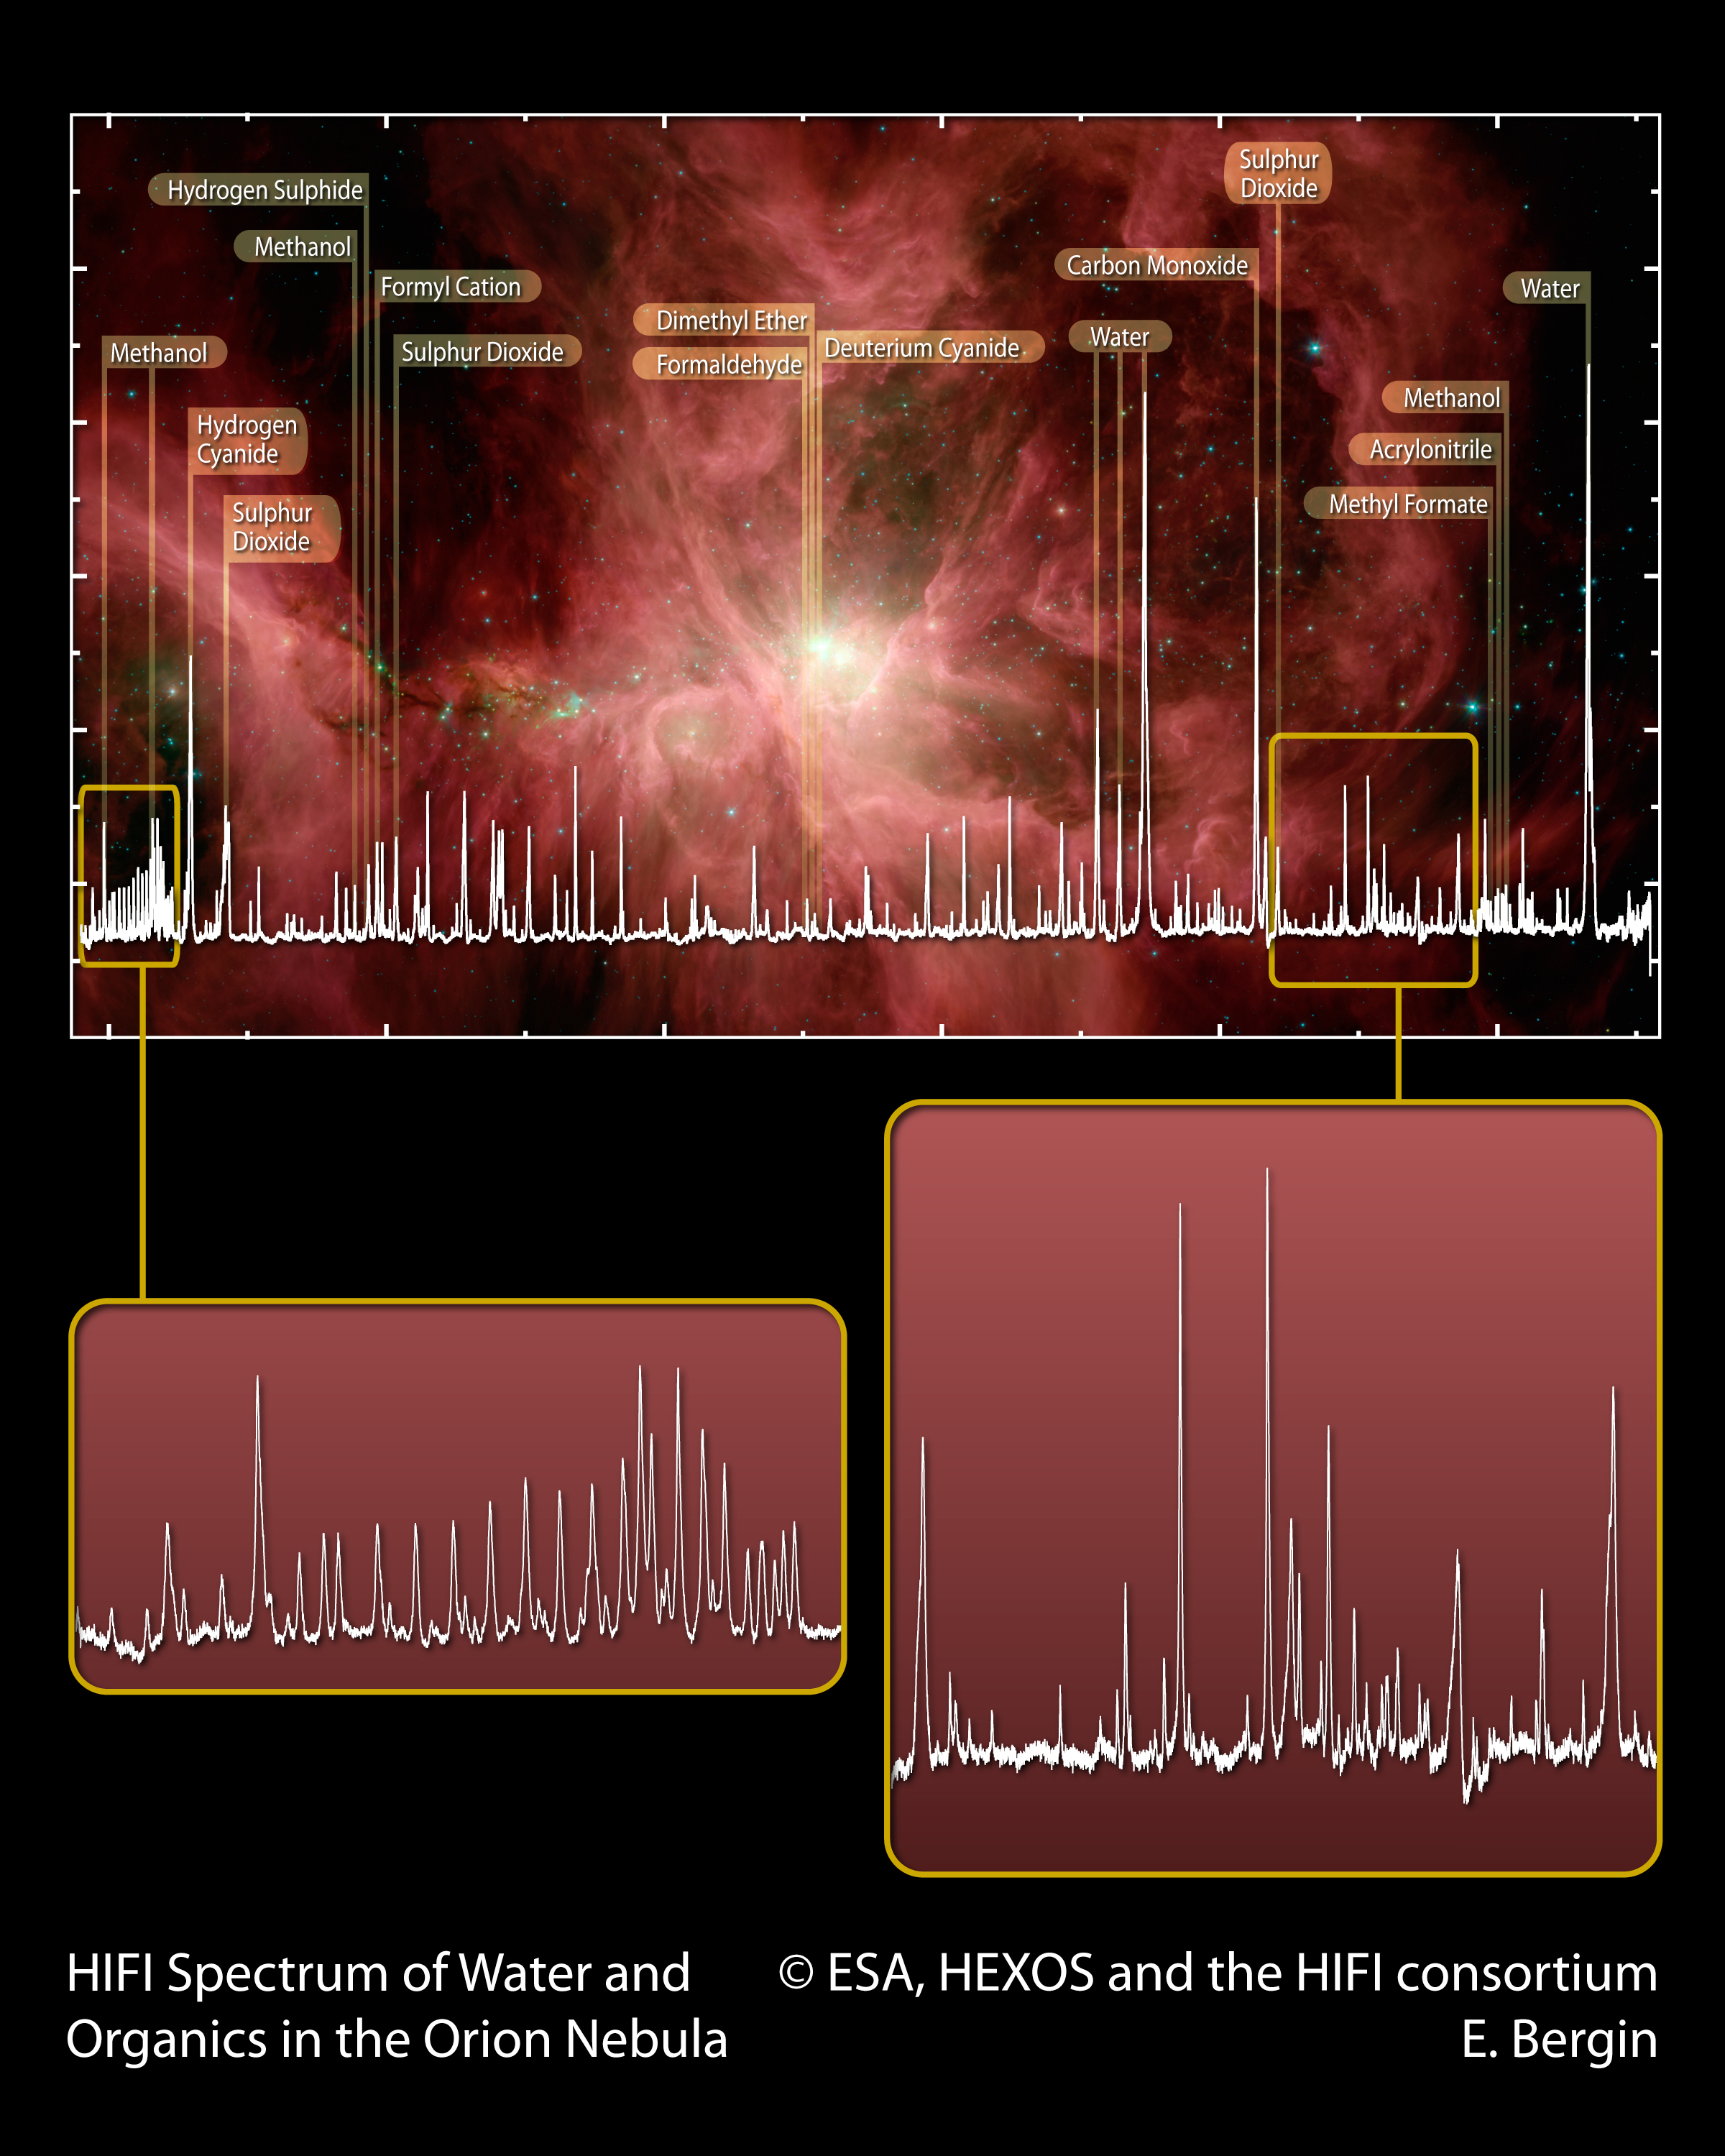
\includegraphics[width=\textwidth]{NHSC_Orion_blowouts_FINAL}
    \caption{HIFI spectrum of the Orion Nebula}
    \caption*{
        The HIFI spectrum of the Orion Nebula,
        superimposed on a Spitzer image of Orion.
        A characteristic feature is the spectral richness: among the organic molecules identified in this spectrum are water, carbon monoxide, formaldehyde, methanol, dimethyl ether, hydrogen cyanide, sulfur oxide, sulfur dioxide and their isotope analogues.
       Copyright: ESA, HEXOS and the HIFI Consortium, 04 March 2010.
    }
    \label{fig:NHSC_Orion_blowouts_FINAL}
\end{figure}

\Cref{fig:NHSC_Orion_blowouts_FINAL} presents the type of spectrum that HIFI can produce.
The axes are not labeled because the picture was released to the press
while the HEXOS\index{HEXOS} team was still analyzing of the data.
The data is now public, and the horizontal axis goes from~\num{1066} to~\SI{1107}{\giga\hertz}, which corresponds to about~\SI{3}{\percent} of the frequency range that HIFI can cover.
The remaining~\SI{97}{\percent} were also measured with that precision.
This spectrum is~\SI{41000}{\mega\hertz}-wide and is taken with a resolution of~\SI{1}{\mega\hertz}, it has therefore~\num{41000}~channels%
\footnote{Actually, \num{82000}~channels because the channels of the WBS are spaced every~\SI{0.5}{\mega\hertz} even though their bandwidth is~\SI{1.1}{\mega\hertz}: the WBS channels overlap somewhat in frequency.}.
Had this spectrum been measured with the most accurate frequency resolution of PACS, it would have less than~\num{200}~channels; most of the spectral features would be blurred, the line profiles would be unresolved, it would be impossible to identify or even detect most of the species and very difficult to determine the kinematics of the gas.




%-----------------------------------------------------------------------------

\subsubsection{A heterodyne receiver}

\index{heterodyne}
The technology that would allow to build a far infrared detector with a spectral resolution of~$10^6$ does not exist yet.
However, detectors with a spectral resolution of \num{5e4} or lower can be built at frequencies of a few gigahertz (microwave region of the electromagnetic spectrum).
This is how HIFI achieves its high spectral resolution: it converts the high-frequency signal from the sky down to a lower frequency, for which high-resolution detectors can be built.
The technique used to lower the frequency of the sky signal is called ``heterodyning''.

A heterodyne receiver creates new frequencies by mixing two frequencies.
The mixing is done by a non-linear device called a ``mixer''\index{mixer}.
In household appliances, the mixer can be a vacuum tube, a diode or a transistor.
In the case of HIFI it is either
a Superconductor-Insulator-Superconductor (SIS) junction that relies on the quantum-tunneling of Cooper pairs of electrons and quasiparticles through the insulator,
or a Hot Electron Bolometer (HEB) that uses the strongly non-linear temperature-dependence of the resistance of a superconductor as a base for the heterodyne mixing process%
~\cite{kooi2008}.
All the mixers of HIFI are cooled to~\SI{1.7}{\kelvin}, the lowest temperature that the Herschel cryostat can provide.
This keeps them in their superconductor state and reduces the thermal noise, which increases their sensitivity.

Typically, the mixer receives two frequencies $f_1$ and $f_2$ and produces two other frequencies $\abs{f_1-f_2}$ and $f_1+f_2$.
One of the two output frequencies is generally discarded, somehow filtered out, while the other is directed toward a detector.
If $f_1$ is the signal we wish to detect, then we can adjust $f_2$ to bring the signal down to the frequency range of the detector.
The frequency that the detector receives is fixed, and called the ``Intermediate Frequency'' (IF).

\begin{figure}[hbtp]
    \centering
    \begin{subfigure}[c]{.7\textwidth}
        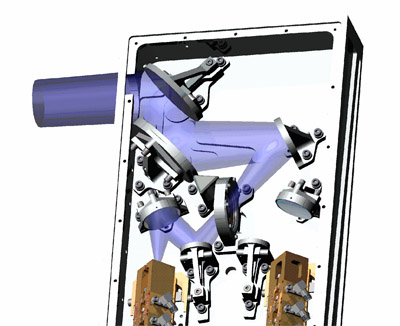
\includegraphics[width=\textwidth]{lou_band_5_drawing}
    \end{subfigure}%
    \begin{subfigure}[c]{.22\textwidth}
        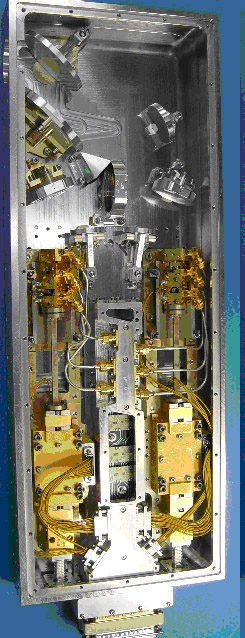
\includegraphics[width=\textwidth]{lou_band_5}%
    \end{subfigure}%
    \caption{The HIFI LO flight model cartridge for Band 5.}
    \caption*{
        The Local Oscillator cartridge contains two signal chains,
        bias filtering modules and an optical system.
        Photo: MPIfR.
    }
    \label{fig:photo_hifi_lou}
\end{figure}

The detectors of HIFI are sensitive to signals between~\num{4} and~\SI{8}{\giga\hertz}.
In other words, the intermediate frequency $f_\text{IF}$ of HIFI is \SI{4}{\giga\hertz}-wide and centered around~\SI{6}{\giga\hertz}.
A Local Oscillator (LO, \cref{fig:photo_hifi_lou}) provides a phase-locked monochromatic signal at a controlled frequency $f_\text{LO}$.
The other signal comes from the sky.
Since $f_\text{IF}$ is fixed, what is the frequency of the sky that we detect for a given LO frequency?
We can answer this question by solving \Cref{eq:heterodyne_question} for $f_\text{sky}$.
\begin{equation}
    f_\text{IF} = \abs{f_\text{sky} - f_\text{LO}} \label{eq:heterodyne_question}
\end{equation}
Because of the absolute value, there are two possible solutions for $f_\text{sky}$ which are given by equations~\eqref{eq:heterodyne_answer_minus} and~\eqref{eq:heterodyne_answer_plus}.
\begin{align}
    f_\text{sky} &= f_\text{LO} - f_\text{IF}
    \text{, or} \label{eq:heterodyne_answer_minus}
    \\
    f_\text{sky} &= f_\text{LO} + f_\text{IF}
    \label{eq:heterodyne_answer_plus}
\end{align}

\Cref{fig:heterodyne_principle} illustrates the heterodyne principle in the case where the output signal at frequency $f_\text{LO}+f_\text{IF}$ is rejected.
\begin{figure}[hbtp]
    \centering
    \input{heterodyne_principle.pdf_tex}
    \caption{The heterodyne principle.}
    \caption*{
        The output of the mixer is a superposition of the lower and upper sidebands of the input, shifted down in frequency.
        Note that the contribution of the LSB is flipped.}
    \label{fig:heterodyne_principle}
\end{figure}

Which one is correct?
In the case of HIFI, both: the detector receives a superposition of the signal coming from two sky frequencies.
This is illustrated on~\cref{fig:heterodyne_principle}.
The frequency $f_\text{LO} - f_\text{IF}$ is called the ``lower sideband (LSB) frequency'' or LSB.
The frequency $f_\text{LO} + f_\text{IF}$ is called the ``upper sideband (USB) frequency'' or USB.
This degeneracy is a problem in HIFI:
does this spectral line belong to the LSB or the USB?
Which fraction of the continuum comes from which sideband?
Answering these questions requires to make assumptions and to know the instrument very well (the mixer gain and optical couplings differs in both sidebands).
There are techniques to deconvolve%
\index{deconvolution}\index{sideband deconvolution}
the sidebands, such as the one presented in%
~\citetitle{comito2002deconvolution} by%
~\citeauthor{comito2002deconvolution}%
~\cite{comito2002deconvolution} which produced the spectrum shown in%
~\cref{fig:NHSC_Orion_blowouts_FINAL}, but they have limitations.

When one listens to a radio program on an analog AM or FM radio receiver, there is no problem with the convolution of the sidebands: if one hears two songs simultaneously, it is because they are broadcast at the same frequency by two nearby but different radio stations, both are in the same sideband.
Radio receivers avoid the sideband convolution by filtering one of the sidebands before mixing.
At radio frequencies, this can be done with a very simple circuit made of a resistor and a capacitor or a coil.
In the far infrared, however, the technology does not exist yet.

If we cannot filter out a sideband, could we separate them somehow?
Sideband-separating mixers do exist.
Once again, this technology was not available at HIFI frequencies when HIFI was designed.
The technology is catching up; ALMA now has sideband-separating mixers in its band 9 cartridges~\cite{mena2007} which operate between \num{600} and \SI{720}{\giga\hertz} (overlapping the low-frequency end of HIFI).
As of 2014, no such mixer exists at higher frequencies.

The sideband convolution was unavoidable when HIFI was designed, and would still be unavoidable if we were designing it now.
It is the price to pay for the high frequency resolution of the instrument.

The determination of the HIFI sideband ratio\index{sideband ratio},
that is the determination of the relative LSB and USB gains of the mixer and the optics,
is still an ongoing effort.
The book that you are reading right now aims at shedding some light on this question.



%-----------------------------------------------------------------------------

\subsubsection{Many instruments in one}
\label{sec:many_instruments_in_one}

No single mixer can cover the HIFI frequency range which extends from~\num{480} to~\SI{1910}{\giga\hertz}.
That frequency range is actually divided into 7 bands listed in~\cref{tab:sevenbands},
each band covering approximately~\SI{200}{\giga\hertz}.
There is a \SI{160}{\giga\hertz}-wide hole in the frequency coverage: band~5 ends at~\SI{1250}{\giga\hertz} and band~6 starts at~\SI{1410}{\giga\hertz}.
\todo{why?}

\begin{table}[hbtp]
    \centering
    \begin{tabular}{ccccc}
        \toprule
        band & freq. range [\si{\giga\hertz}] & LO injection & mixer & coupling \\
        \midrule
        1 &  480--640  & beam splitter & SIS & horn\\
        2 &  640--800  & beam splitter & SIS & horn\\
        3 &  800--960  & diplexer      & SIS & horn\\
        4 &  960--1120 & diplexer      & SIS & horn\\
        5 & 1120--1250 & beam splitter & SIS & lens\\
        6 & 1410--1703 & diplexer      & HEB & lens\\
        7 & 1703--1910 & diplexer      & HEB & lens\\
        \bottomrule
    \end{tabular}
    \caption{Frequency and technology of the seven HIFI bands.}
    \label{tab:sevenbands}
\end{table}

HIFI is more like 7 independent instruments.
Two mixer technologies (SIS and HEB, with different materials for the SIS),
two focusing technologies (lenses and horns),
two LO-injection methods (beam splitter and diplexers),
all mixed.

That 7 is multiplied by 2 when we consider that each band separates the incoming sky signal into two linear polarizations, which we conventionally name H and V, for ``horizontal'' and ``vertical''.
Each band has a mixer for H and a mixer for V.

Furthermore, each band requires two local oscillators, each able to pump the mixers in half of their frequency range.
The local oscillators for each band are labeled with the letters ``a'' and ``b''.
An observation in band~5a means that we use the band~5 mixer with its lower-frequency-end local oscillator.
\Cref{fig:photo_hifi_lou} illustrates this: there are two apparently identical sources (in yellow) but only one output (blue beam exiting on the left).
A local oscillator, whether a or b, pumps the H and V mixers of its band simultaneously.

Finally, each polarization has two backends.
Backends are the microwave detectors placed after the mixer.
The Wideband Spectrometer (WBS) is an acousto-optic detector; it covers the full IF from \num{4} to \SI{8}{\giga\hertz} with 8192 channels of \SI{1.1}{\mega\hertz} or resolution\todo{citation}.
The High-Resolution Spectrometer (HRS) is a digital autocorrelator; its 4080 channels can be allocated to satisfy various bandwidth/resolution trade-offs\todo{citation}.
For reason of redundancy, the WBS-H and WBS-V backends are identical but independent, so are the HRS-H and HRS-V.

\Cref{eq:hifi_56} should make clear that HIFI is a complex instrument.
\begin{equation}
    7 \text{ mixers}
    \times
    2 \text{ LO's}
    \times
    2 \text{ polarizations}
    \times
    2 \text{ backends}
    =
    56 \text{ combinations}
    \label{eq:hifi_56}
\end{equation}
\begin{figure}
    \centering
    \begin{subfigure}[c]{.4\textwidth}
        \includegraphics[width=\textwidth]{hifi_fpu}
    \end{subfigure}%
    \begin{subfigure}[c]{.6\textwidth}
        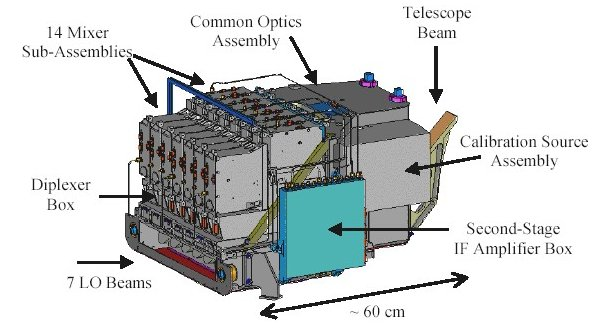
\includegraphics[width=\textwidth]{hifi_fpu_schematic}
    \end{subfigure}
    \caption{HIFI FPU.}
    \caption*{Photograph of the focal plane unit (FPU) of heterodyne instrument for the far infrared (HIFI).  Photo: ESA 2007.}
    \label{fig:photo_hifi_fpu}
\end{figure}
\Cref{fig:photo_hifi_fpu} shows the focal plane unit (FPU) of HIFI.
The sky signals enters the instrument on the right side.
On the left side, in red, are the seven windows that are facing the seven local oscillator cartridges.
The FPU is inside the cryostat but the local oscillators are not.
The seven windows in the cryostat are visible on~\cref{fig:photo_hifi_cryo}: 9 holes for 7 local oscillator beams and 2 alignment devices, lined-up horizontally toward the top of the tank.
\Cref{fig:photo_hifi_fpu} also shows the 14 mixer units: 7 on the left above the LO feeds for one polarization, and 7 on top for the other polarization.

In this book, we will focus on the SIS bands (1 to 5) and the WBS backend,
leaving ``only'' 20 instrumental configurations to explore.
The reasons for focusing on SIS and WBS will become clear in the next section, in which we introduce the problem that HIFI has with standing waves.

\todo[inline]{Refer to~\cite{AA_537_A17} somewhere.}


%=============================================================================
\section{Standing waves in HIFI}

\subsection{Ripples on spectra}
Despite the careful design of HIFI, its spectra can show ripples.
A somewhat extreme example is given on~\cref{fig:mars_50010cb7_WBSH_USB}.
The baseline of this spectrum of Mars should be flat, but instead shows a strong ripple that has a period of about~\SI{100}{\mega\hertz}.
This is an instrumental artifact that was not removed during the calibration.
We will discuss in details the calibration of HIFI in%
~\cref{sec:chapter4}.

\begin{figure}[htbp]
    \centering
    \includegraphics[width=.8\textwidth]{mars_50010cb7_WBSH_USB}
    \caption{Continuum and absorption line of Mars with ripples.}
    \caption*{
        HIFI spectrum taken from the observation ID 0x50010cb7.
        The baseline of this spectrum, which corresponds to the continuum emission of the planet, should be flat.
        Its periodic modulation indicates the presence of cavities in the optical system, the effect of which was not calibrated out.
    }
    \label{fig:mars_50010cb7_WBSH_USB}
\end{figure}

Often, the ripples are weaker.
Many factors influence which ripples will show and with which intensity: LO frequency, LO mode (resistor or varactor), mixer bias, diplexer tuning, and of course the power of the astronomical signal, of the calibration loads black body radiation and of the LO.
HIFI being heterodyne, the ripples in the LSB and those of the USB can interfere destructively.
As we will show in~\cref{sec:chapter5}, the fact that we do not see a ripple does not mean that the data is not affected.
Indeed, the line profile can be distorted even though the baseline appears flat.


%-----------------------------------------------------------------------------
\subsection{Cavities cause ripples}
Ripples are due to an instrumental artifact that the calibration does not compensate.
Some surfaces in the instrument reflect the signal away from the mixer, reducing the coupling of the mixer to that signal.
Other surfaces reflect that reflected signal back toward the mixer, increasing the coupling again.
The electromagnetic waves go back and forth between all the optical elements and interfere with each other.
The combined effect these infinite reflections depends on the distances between these elements, their surface properties, and the wavelength of the signal.

This dependence on the wavelength explains the periodicity ripples.
Any pair of reflective surfaces that can `see' each other is called a cavity.
The period of a ripple is linked to the ratio of the wavelength and the length of the cavity.

\begin{figure}[hbtp]
    \centering
    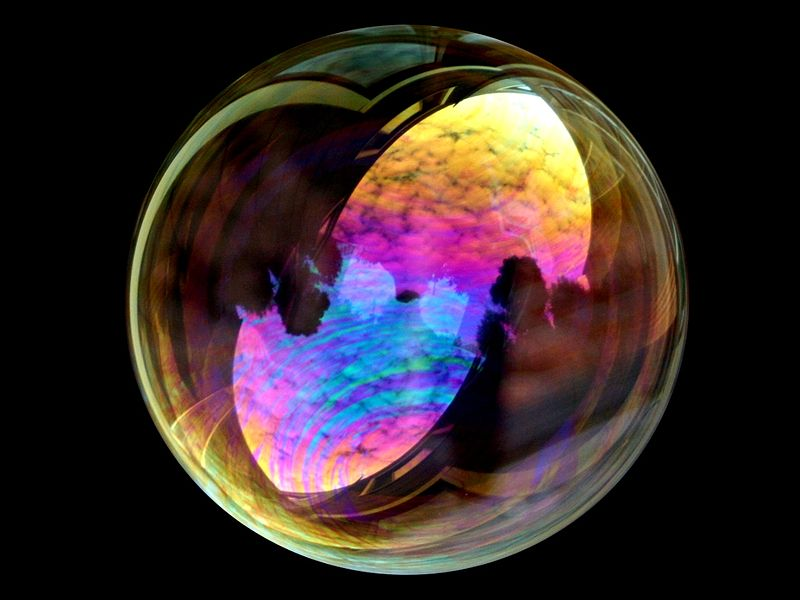
\includegraphics[width=.8\textwidth]{soap_bubble_sky}
    \caption{Interferences in a thin film of soap.}
    \label{fig:soap_bubble}
\end{figure}

\Cref{fig:soap_bubble} illustrates the wavelength-dependence of the effect of a cavity in a familiar case: that of the iridescence of a soap bubble.
The thickness of the thin layer of soap at any given point, combined with the direction of propagation of the light at that point, determines which wavelengths will interfere positively or destructively in the direction of your eye.
The spectrum reflected and transmitted by the bubble is profoundly modified by the soap cavity, and the eye sees many colors as a result.

Cavities exist in the optical path of HIFI.
For example, the mixer and the local oscillator form a cavity.
So does the mixer and the calibration cold black body, or the mixer and the roof-top mirrors of the diplexer units (more on these in~\cref{sec:chapter3}).
Any pair of surface that somehow face each other, even via other surfaces, form a cavity.
There are also cavities in the microwave side of HIFI: after the mixer.
The bands 6 and 7 of HIFI lack isolators between the mixer and the IF-amplifiers.
This allows the mixer to see the amplifier and creates a cavity.
The case of the interferences on the IF-side of the mixer in bands~6 and~7 has been investigated by~\citeauthor{higgins2011} in the chapter 3 of his Ph.D.\ thesis \citetitle{higgins2011}~\cite{higgins2011}.
In the present book, we will focus on the optical side.

The \cref{sec:chapter2} will detail how cavities work, how they give raise to standing waves, and how they create ripples on the spectra by modulating the efficiency of the optical system.
The reason why cavities are a problem in HIFI and not in other instruments is because HIFI is a coherent receiver.

%-----------------------------------------------------------------------------
\subsection{Coherence necessary for interferences}
\label{sec:hifi_is_coherent}

Not every instrument is sensitive to the effect of cavities in its optical path.
The soap bubble of~\cref{fig:soap_bubble} presents obvious signs of interferences, but when we look through a glass window there are none.
Why would a layer of soap and a layer of glass behave differently?
Obviously, the refractive index is not the same for soap and for glass, but this is not the reason.

For a cavity to give rise to interferences, the cavity must be short when compared to the coherence length\index{coherence length} of a wave.
A soap bubble is about~\SI{1}{\micro\meter}-thick, while a glass pane has a typical thickness of~\SI{5}{\milli\meter}.
The difference of behavior between the two resides in the thickness.

For an electromagnetic wave, the coherence time is the time over which a propagating wave may be considered coherent.
In other words, it is the time interval within which its phase is, on average, predictable.
The coherence length equals the coherence time multiplied by the speed of the wave in the medium.

The coherence time, or coherence length, is a function of the bandwidth of the signal.
The coherence time~$\tau$ of a signal is inversely proportional to its bandwidth~$\Delta f$.
This is illustrated in~\cref{fig:coherence}, and~\cref{sec:chapter2} will review it in more details.
\begin{figure}[hbtp]
    \centering
    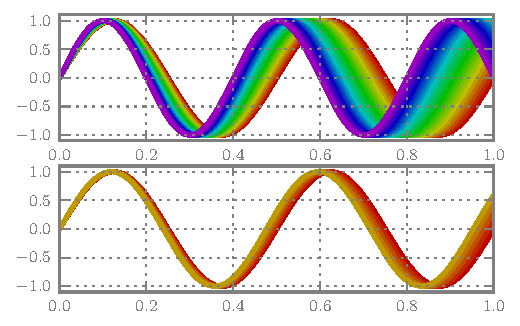
\includegraphics[width=.8\textwidth]{coherence}
    \caption{Coherence time depends on bandwidth}
    \caption*{
        Signals with a narrow bandwidth remain in phase longer.
        Colors represent frequencies.
        The $x$ axis can represent either time or space and the $y$ axis represents the amplitude of the electric field for the corresponding frequency, both in arbitrary units.
        After propagating to $x=0.85$, the red and purple frequencies of the top-plot signal have opposite phase; a detector that cannot discriminate between them adds up their contribution to 0.
        In the bottom plot, the signal is still very much in phase at $x=0.85$
        because it has a narrower bandwidth.
    }
    \label{fig:coherence}
\end{figure}

When cavities are short enough compared to the coherence length of a wave, then the wave remains coherent during its trips back and forth between the two surfaces.
This allows the wave to interfere with itself.
There is no interference without coherence.

Each WBS channel has a bandwidth $\Delta f = \SI{1.1}{\mega\hertz}$,
which yields $\tau = 1 / \Delta f = \SI{909}{\nano\second}$.
By multiplying by the speed of light, we find that the WBS has a coherence length of~\SI{273}{\meter}.
This means that, as long as a signals travels significantly less than~\SI{273}{\meter}, it is coherent as far as the WBS is concerned.
The path lengths inside HIFI are much shorter than~\SI{273}{\meter}.
For example, the distance between the LO and the mixers is about~\SI{1}{\meter}.
In that context, all the sources of noise in HIFI are coherent.

%-----------------------------------------------------------------------------
\subsection{Standing waves}
Standing waves are a side-effect of coherence and cavities.
When light enters a cavity, some of the light is reflected, some of the light is transmitted, some of the light is lost (heat) and some of the light is stored inside the cavity.

The light stored inside the cavity can be seen in two ways:
either as a superposition of an infinity of waves traveling in both directions,
or as a single wave that is not traveling.
Both interpretations are equally valid, both are solutions to Maxwell's equations.
It is a matter of perspective.
When we consider the light trapped in the cavity as a single wave, its nodes and crests do not move: the oscillation stands there, fixed in space.
This is what we call a ``standing wave''.

Astronomers and engineers alike tend to abuse the language slightly for the sake of brevity and because the context is often clear.
Some would say that the spectrum shown in~\cref{fig:mars_50010cb7_WBSH_USB} has a standing wave, using the word ``standing wave'' to mean ``ripple''.
Some would say that standing waves are responsible for the ripple, using ``standing wave'' instead of ``interferences''.

In truth, both the ripples and the standing waves are the result of interferences.
The ripple is a frequency-dependent modulation of the light exiting the cavity, and the standing wave corresponds to the light that remains in the cavity for a given frequency.
The three concepts ``ripple'', ``standing wave'' and ``interference in a cavity'' are tightly coupled and go together, one cannot have one without the others.
This is why this slight abuse of language is acceptable.
However, for the sake of clarity, we will carefully choose our words in the rest of this book.


%=============================================================================
\section{The chapters of this book}

\Cref{sec:chapter2} will dive into the physics and mathematics of coherence, cavities, standing waves and interferences.
After an introduction to cavities, we introduce a novel approach to modeling interferences in cavities.

This model has two aspects.
The first aspect is a solver: a set of formulas and algorithms that take optical elements described with matrices, and predicts the coupling efficiency of every element to a source.
It solves directly for the steady state and takes into account the infinity of reflections between every possible pair of elements along every possible path.

The second aspect of the model is a library: a set of formulas and algorithms that produces matrices describing optical elements such as rooftop mirrors, wire grid polarizers or thin film beam splitters.
These matrices are fed to the solver.

The method presented in \cref{sec:chapter2} can be applied to any coherent instrument, not only HIFI, as long as it satisfies some conditions.

In \Cref{sec:chapter3}, we use the model described in \cref{sec:chapter2} to build a numerical model of a band of HIFI.
We then explore the many parameters of the model, starting from an ideal and perfect instrument and making it more and more realistic.
This approach reveals the parameters that are the most important in giving rise to ripples.

The spectral features reproduced by the model in this chapter match qualitatively many features observed on real HIFI data.
This indicates that the method described in~\cref{sec:chapter2} can be used during the design phase of an instrument.
Whether standing waves are desired or not in the instrument, the model can predict them, at least quantitatively.

With~\cref{sec:chapter4}, we attempt to push the model further by trying to reproduce some HIFI data quantitatively.
The goal is to predict the value of some efficiencies that appear in the calibration equations and that cannot be determined any other way.
Constraining these efficiencies would allow the calibration to get rid of the ripples.
Determining these parameters proves to be a difficult task, especially when this is done after the end of the mission.
Future instruments may have more success by performing some dedicated tests and observations.

Finally, \cref{sec:chapter5} explores the impact of interferences in HIFI on the estimation of the physical parameters of a star forming region.
This chapter translates an uncertainty on the amplitude of a line into an uncertainty on the temperature and pressure of a cloud.





%###############################################################
% IMPORTED FROM CHAPTER 2, NEEDS TO BE MERGED.
\subsection{The importance of calibrating and modeling instruments}

Microscopes, mass spectrometers, hourglasses, seismographs, measuring tape, magnetic resonance imagine scanners, telescopes, 
we build instruments to measure parameters and properties of the objects and events around us.

The more accurate the instrument, the more precisely we can constrain the value of these physical parameters.
With enough precision, we can confirm of infirm hypotheses, reinforce theories or find their limitations, and advance science.
Noise and imperfections in our instruments obviously limit the precision that we can achieve and hinder scientific progress.

There is another source of uncertainty: we do not always know well enough how our instruments behave.
Even an instrument built perfectly according to specifications, perfectly protected from exterior perturbations and maintained perfectly stable can behave in ways that we do not understand fully.
We call ``external parameters'' the physical parameters of the phenomenon that we wish to study,
and we call ``internal parameters'' the physical parameters of the instrument itself.
In mathematical terms, the transfer function~$F$ of an instrument often involves internal parameters for which the value is not well known at the moment of the observation.
\begin{equation}
    y = F(x, p_0, p_1, p_2, p_3, p_4, \dots)
\end{equation}
The transfer function~$F$ can be (very) complicated and is often non-linear.
When we invert $F$ to retrieve the real value $x$ of an external parameter from the value $y$ that we measured, any unknown internal parameter $p_i$ adds to the uncertainty.
When we wish to reduce the uncertainty, we have two possible courses of action.

The first possibility is to take measurements of well known reference sources: we assume that~$x_j$ is known, where~$j$ identifies a specific source.
With enough $(x_j, y_j)$ tuples we can constrain the relations between the internal parameters~$p_i$.
This is called ``calibrating the instrument''.
The time scale upon which the internal parameters drift determines how often we must recalibrate it.

The second possibility is to calculate the value of these unknown internal parameters by modeling the physics that happens inside the instrument.
For example, how the temperature of an instrument contracts or expands its optical lenses can in principle be computed.

Why would we ever go through the troubles of modeling parameters when we can `simply' measure them with calibration measurements?
There are many reasons.
The time spent calibrating the instrument is not spent measuring interesting things.
There may just be too many parameters.
The instrument might not even exist anymore, and we are left with an archive of data that might or might not contain the observation you need to determine the value that parameter $p_7$ had in December three years ago.

\subsection{Focus on the optics of HIFI}

This chapter describes the result of our efforts to model electromagnetic interferences in a coherent high-resolution spectrometer.
The Heterodyne Instrument for the Far Infrared (HIFI)~\cite{AA_518_L6} is a state-of-the art high-resolution spectrometer designed for the study of the chemistry and dynamics of a wide range or astrophysical environment such as star forming regions, galactic evolution and planetary atmospheres.
HIFI operates between~\num{640} and \SI{1910}{\giga\hertz}, a frequency range that is covered by seven bands.
The absolute calibration accuracy of HIFI is at least~\SI{10}{\percent}, with a goal of~\SI{3}{\percent}.
\Cref{tab:calibration_errors} summarizes the origin of the actual calibration uncertainties for the seven bands.
The sideband ratio and the optical standing waves stand out in this table for being amongst the biggest contributors to the uncertainty.

\begin{table}[hbtp]
    \centering
    \begin{tabular}{lcccc}
        \toprule
        Error source           & Band 1/2 & Band 3/4 & Band 5 & Band 6/7 \\
        \midrule
        Sideband ratio         & 3--4     & 4--6     & 4--6   & 5--8     \\
        Hot load coupling      & <1       & <1       & <1     & <1       \\
        Cold load coupling     & <1       & <1       & <1     & <1       \\
        Hot load temperature   & <1       & <1       & <1     & <1       \\
        Cold load temperature  & <1       & <1       & <1     & <1       \\
        Planetary model error  & <3       & <3       & <3     & <3       \\
        Beam Efficiency        & <5       & <5       & <10    & <5       \\
        Pointing               & <1       & <2       & <2     & <4       \\
        Optical standing waves &  4       & 4        & 3      & 3        \\
        \bottomrule
    \end{tabular}
    \caption{Overall error budget of HIFI.}
    \caption*{
        This tables provides the percentage flux error associated with each component of the error budget.
        Source: \citetitle{hifiobserversmanual}~\cite{hifiobserversmanual}.
    }
    \label{tab:calibration_errors}
\end{table}

In HIFI, the problem of the sideband ratio and that of standing waves are actually related.
Both are influenced by the optics of the instrument.
Let us explain these terms in a few words.

\subsubsection{The sideband ratio}
HIFI is a heterodyne spectrometer.
Heterodyne spectrometers are sensitive to two ranges of frequencies simultaneously.
These frequency ranges are called ``sidebands''; the sideband with the lowest frequencies is called ``lower sideband'' (LSB), and the other ``upper sideband'' (USB).
A heterodyne spectrometer overlaps these two sidebands and returns a single measurement value~$y$, as shown in~\cref{eq:explain_sbr_0}.
\begin{equation}
    y = G_\text{LSB} b_\text{LSB} + G_\text{USB} (b_\text{USB} + x)
    \label{eq:explain_sbr_0}
\end{equation}
Often, the source of interest emits radiation in one sideband only.
In our equation, we assumed that the source emits a power~$x$ in the USB.
The other sideband receives whatever background radiation~$b$ is emitted at that time.
The background radiation is usually well known, our real unknown is~$x$.
Our problem comes from the fact that the gain of the instrument in the LSB ($G_\text{LSB}$) is different from the gain in the USB ($G_\text{LSB}$).

Let us rewrite the previous equation in a way that explicitly shows the imbalance between the sidebands.
\begin{equation}
    y =
    (G_\text{LSB} + G_\text{USB})
    \bigg( (1-g) b_\text{LSB} + g (b_\text{USB} + x) \bigg)
    \label{eq:explain_sbr_1}
\end{equation}
Here, $g = G_\text{USB}/(G_\text{LSB} + G_\text{USB})$ and is called ``sideband ratio''.
The sideband ratio equals 0.5 when the detector is balanced.

It is relatively easy to calibrate the value of total gain $G_\text{LSB} + G_\text{USB}$:
just observe at a point in the sky for which $x=0$.
However, calibrating the sideband ratio~$g$ is not easy: it is actually a combination of many instrumental parameters.

There are two contributions to the sideband ratio: the mixer gain, and the coupling of the mixer to the source.
In this book, we are interested in the second contribution: the coupling of the mixer to the source.
We want to model the effect that the optics of HIFI has on its sideband ratio. 

\subsubsection{Standing waves}
Another considerable source of uncertainty in HIFI, according to~\cref{tab:calibration_errors}, is the presence of standing waves in the optics.
Standing waves refer to electromagnetic waves trapped between reflective surfaces in an instrument.
They are a result of an electromagnetic wave interfering with itself.
These interferences modulate the coupling of the mixer to the source.
They also modulate the coupling of the mixer to the sources that are used for calibration, but they do it differently, so they cannot be calibrated out.
Here as well, modeling the optics should predict the loss of coupling due to interferences.

\subsubsection{Coherence}
The channels of HIFI have a bandwidth of~\SI{1.1}{\mega\hertz} or lower.
When the bandwidth is so narrow, the thermal noise of the astronomical source, the calibration black bodies and the local oscillator (LO) qualify as ``narrow band Gaussian noise signals''~\cite{siegman1986lasers}.
They have a coherence time~$\tau$ equal to the inverse of their bandwidth~$\tau=1/\Delta f$.
A bandwidth of~\SI{1}{\mega\hertz} results in a coherence time of~\SI{1}{\micro\second} equivalent to a coherence length of~\SI{300}{\meter}.
This is a hundred times the longest distance inside HIFI.
Therefore, in HIFI, the signals from the LO, the calibration sources and the sky are coherent.

The notion of coherence refers to the degree of correlation, described in a specific mathematical fashion, between two signals observed at different points in time and/or space.
The amplitude, the phase and the polarization of the electromagnetic waves inside HIFI change only slowly with time.
The amplitude, phase and polarization of the wave at any one time is strongly correlated with the amplitude phase and polarization of that same wave at considerably earlier or later times.
Between these two moments, the wave may have undergone several reflections on the various optical elements that make the instrument.
These reflections can make the wave overlap itself in space, and the strong degree of phase correlation implies that the wave interferes with itself.

Reflections in a coherent system give rise to interferences, and interferences inside a cavity create standing waves.
Any two surfaces that face each other via at least one optical path form a cavity.
The cavity formed by the detector and the secondary mirror is one that is often considered during the design of a telescope.
Other cavities exist inside HIFI: the mixers, local oscillators, calibration loads, diplexer roof-top mirrors, beam splitters, are all surfaces that somehow face each others.

In his technical note from~\citedate{whyborn2002standingwaves} entitled
\citetitle{whyborn2002standingwaves},
\citeauthor{whyborn2002standingwaves} mentions that standing waves can not only modulate the optical coupling between a source and a detector (as we will spend the rest of this chapter exploring), but also the intrinsic noise of the mixer itself.
We are not going to cover that second point.
In this chapter, we focus on modeling the interferences in the optical path.

\subsection{Why a new technique?}
Because the far-infrared is between the microwave and optical domains of the electromagnetic spectrum, many modeling techniques developed for microwave or optical engineering can be applied to the far-infrared.
However, no technique exists that can deal with both the optical and the microwave aspect at the same time.

From the optical side, we can use ray tracing~\cite{spencer1962general}.
Ray tracing often assumes that the light is incoherent and propagates along infinitely-thin beams.
Laser theory introduces some tools to deal with coherence and the self-diffraction of the beam~\cite{siegman1986lasers}.
These theories make use of matrices to describe changes to the degree of polarization of light (Stokes parameters, Müller matrices, Jones matrices), and to the geometry of the beam (ray optics or Gaussian beams ABCD matrices)~\cite{goldsmith1998quasioptical}.

From microwave circuits and waveguides theory, we can use the many types of 2--by--2 matrices that link voltage and current for two-ports networks: there is a homomorphism between \{voltage, current, relations between them\} and \{electric field, magnetizing field, relations between them\}.
There are also scattering matrices which allow for more than two ports~\cite{pozar2009microwave}.

\Cref{tab:tools} presents a brief overview of different tools used to model optical or microwave systems.
We will not describe them all.
Suffice to say that there is no magic bullet that treats all the aspect of the problem at once.
Some tools are designed explicitly to model polarization for example, others can be tweaked in order to include it, and other tools again are just not made for that.

In this chapter, we are not proposing a such magic bullet.
We are going to combine several techniques inspired from circuit theory (notably scattering and Jones matrices), extend them to work in three dimensions, and show how to solve the steady state of optical systems of any size and complexity.
For now, we are ignoring the geometry of the beam: we assume that our waves are plane and our signals are mono-modes.
This is a first-order approximation that lets us focus on the intensity, phase and polarization coherence of these waves.

\begin{sidewaystable}[hbtp]
    \centering
    {\footnotesize
    \rowcolors{1}{gray!20}{}
    \begin{tabularx}{\textwidth}{X|X X X X X X}
        \toprule
                                          & Ray tracing & Ray optics ABCD matrix & 2-port network matrices & Scattering matrix & Jones matrix & Müller matrix  \\
        \midrule
        Intensity/power                   & yes         & no                     & yes                     & yes               & yes          & yes            \\
        Phase (coherence)                 & yes         & yes                    & yes                     & yes               & yes          & no             \\
        Polarized                         & yes         & possible               & irrelevant              & possible          & yes          & yes            \\
        Unpolarized                       & yes         & yes                    & irrelevant              & possible          & no           & yes            \\
        Direction of propagation          & yes         & a bit                  & no                      & no                & no           & no             \\
        Gaussian beam width and curvature & no          & yes                    & no                      & no                & no           & no             \\
        Gaussian beam modes               & no          & yes                    & no                      & no                & no           & no             \\
        More than 2 ports                 & yes         & no                     & no                      & yes               & no           & no             \\
        Cascade-able                      & yes         & yes                    & some                    & no                & yes          & yes            \\
        Steady-state                      & no          & no                     & yes                     & yes               & no           & no             \\
        \bottomrule
        \end{tabularx}
    }
    \rowcolors{1}{}{}
    \caption{\label{tab:tools}No tool or framework satisfies all the criteria.}
\end{sidewaystable}


%###############################################################
% IMPORTED FROM CHAPTER 4, NEEDS TO BE MERGED.

%=============================================================================
\section{Introduction}

Measuring a physical phenomenon often requires converting one physical quantity into another.
For example, a mercury-in-glass thermometer converts a temperature~$T$ into a length~$L$.
The mathematical function linking these two quantities can be more or less well known, and may depend on any number of parameters.
In the case of the thermometer, we can assume an affine relationship $L = aT+b$, where~$a$ and~$b$ are a priori unknown.
Calibrating the instrument consists in determining the values of the parameters so that we can solve the equation to retrieve the original physical quantity.
In order to calibrate our thermometer, we could walk to a beach (where the atmospheric pressure is \SI{100}{\hecto\pascal}).
Plunging our thermometer in melting ice gives us~$L$ for $T=\SI{0}{\degreeCelsius}$.
Plunging it in boiling water gives us~$L$ for $T=\SI{100}{\degreeCelsius}$.
From these two measurements, calculating~$a$ and~$b$ is trivial and we can start graduating the glass.

The calibration of a telescope follows a similar principle.
A telescope, whether radio, optical or gamma, converts the power of the electromagnetic radiation into digitized ``counts'', the nature of which depend on the backend.
The backend can be a CCD camera for instance.
Astronomical signals are often very weak compared to other sources of radiation, like the atmosphere, the telesope itself, or even the background radiation from the sky.
One goal of the calibration is to remove this unwanted contribution and isolate the signal coming from the source.
In the example of our thermometer, this step corresponds to determining the parameter~$b$.
The second step of the calibration consists in converting the signal from the source, expressed in backend counts, into the physical unit that we try to measure.
This step corresponds to determining the value of the parameter~$a$.

In their famous article \citetitle{ulich1976absolute} \cite{ulich1976absolute}, \citeauthor{ulich1976absolute} describe the merit of the ``chopper-wheel'' calibration method.
This methods consists in tilting a mirror to couple the beam of the telescope either to the sky or to calibration sources.
The power radiated by these calibration sources is known, which allows the determination of the unit-conversion factor at the moment of the observation.
For an instrument like HIFI, the Heterodyne Instrument for the Far infrared this method needs to be extended.
Indeed, as we described in~\cref{sec:chapter1}, HIFI is a coherent and double-sideband detector.
This complicates the calibration equations by introducing several parameters coping with both sidebands and the various interferences.

In the following section, we describe the calibration equations used for HIFI, with their strengths and limitations.
Then we explain how our method for modeling interferences, which we described in~\cref{sec:chapter2}, could predict the value of some parameters of these calibration equations, thereby reducing the uncertainties on the final spectrum.

Finally, in~\cref{sec:matching_the_model_to_the_data}, we take the first step toward putting our theory into practice.


%=============================================================================
\section{HIFI calibration}
\label{seq:hifi_calibration}

%-----------------------------------------------------------------------------
\subsection{Introduction}
The absolute intensity calibration of HIFI relies on the chopper wheel method \cite{ulich1976absolute}, with calibration loads, modified to accomodate the double-sideband and coherent nature of HIFI.

In this section, we will briefly present the chopper mechanism and the calibration loads of HIFI.

Then, we explain the calibration equation, the purpose of the reference subtraction and the bandpass measurement, and whether or not it properly takes into account the interferences that occur in the optical path of the instrument.

Since there are not always a reference position on the sky to which HIFI can quickly chop, 
there are HIFI several observing modes, which differ by their choice of reference.
Each observing mode has its own impact on interferences.

Finally, we dive into the details of the calibration equations and show precisely which parameters our interference model should predict.

%-----------------------------------------------------------------------------
\subsection{HIFI chopper and calibration source assembly}

The chopper of HIFI (\cref{fig:chopper_angles}) is an actuated mirror that can rotate around one axis to direct the beam anywhere within a \SI{15}{\degree} range.
Inside that range are positions of interests: the two calibration loads and the sky, as shown in~\cref{tab:chopper_angles}.
More information about the chopper can be found in~\citetitle{huisman2011cryogenic}
by~\citeauthor{huisman2011cryogenic}~\cite{huisman2011cryogenic}.

\begin{table}[hbtp]
    \centering
    \begin{tabular}{Sl}
        \toprule
        \multicolumn{1}{l}{chopper angle [\si{\degree}]} & HIFI beam direction \\
        \midrule
        -4    & endstop \\
        -2.45 & \SI{-1.5}{'} on the sky \\
         0    & \SI{0}{'} on the sky \\
         2.45 & \SI{1.5}{'} on the sky \\
         8    & cold calibration load \\
        10.4  & hot calibration load \\
        11.0  & endstop \\
        \bottomrule
    \end{tabular}
    \caption{Relation between the chopper angle and the direction of the HIFI beam.}
    \label{tab:chopper_angles}
\end{table}
\begin{figure}[hbtp]
    \centering
    \includegraphics[width=\textwidth]{beam_and_chopper_rotations}
    \caption{Drawing of the chopper mechanism and its angles.}
    \label{fig:chopper_angles}
\end{figure}

\Cref{fig:hbb} shows the hot calibration source of HIFI, also refered to as ``hot black body'' or HBB.
The HBB source is heated to~\SI{100}{\kelvin} and is isolated from its~\SI{10}{\kelvin} by being suspended by wires.
The HBB is wedge-shaped and is coated in \ce{SiC}~foam.
Its aperture is rectangular to accomodate the direction of incidence of the seven beams from the seven HIFI bands.

The cold calibration source, or ``cold black body'' or CBB, has a simpler design.
It consists in a flat surface of the \SI{10}{\kelvin} aluminum casing of HIFI that is covered in \ce{SiC}~foam.
It is tilted relatively to the incoming beam in order to prevent any reflection from coming back.

\ce{SiC} is~\SI{95}{\percent} emissive \cite{klaassen2003scattering}.
The remaining~\SI{5}{\percent} of reflection are scattered by the roughness of the foam surface.

\begin{figure}[hbtp]
    \centering
    \input{hbb.pdf_tex}
    \caption{The Hot Black Body calibration source of HIFI.}
    \label{fig:hbb}
\end{figure}

Despite being called ``black bodies'', the calibration load of HIFI are not perfect absorbers:
since the coating scatters the light in random directions, some of it can go back into the beam.
In~\cref{sec:matching_the_model_to_the_data}, we will attempt to measure their coefficient of reflection at~\SI{491}{\giga\hertz}.

%-----------------------------------------------------------------------------
\subsection{Reference subtraction}
The goal of the reference subtraction is to remove the background noise originating from the telescope itself.
Indeed, its primary mirror has a temperature of about \SI{80}{\kelvin} \cite{Sein2004mirror}.
The local oscillator is also a source of noise of about \SI{120}{\kelvin}.
Finally, the focal plane unit of HIFI itself has a temperature of about \SI{10}{\kelvin}.
Subtracting the signal received from a reference point in the sky that is devoid of emission actually cleans the spectrum taken on the source from all these noise contributions.
This works only if the instrument does not change significantly between the integration on the source and that on the reference.
Possible changes are thermal instabilities and deliberate changes in the optical paths resulting from the actuation of the chopper or the diplexers.

Subtracting spectra taken with different optical paths can result in visible distortions of the calibrated spectrum, notably in the form of ripples on the baseline.
These ripples are a result of interferences.
Interferences modulate both the astronomical signal and the background noise.
The background noise has often much more power than the astronomical (line and/or continuum) signal.
Because the noise is so powerful, even a relatively small residual due to a minute change in interferences can have an absolute level commensurable with that of the astronomical signal.
For example, a \SI{100}{\kelvin} noise that differs by only \SI{1}{\percent} between the Source and Reference spectra leaves a \SI{1}{\kelvin} residual on the calibrated spectra, which is very significant in many observations.

There is one important point to remember here: even the best reference source in the universe cannot correct for the effect of the interferences on the useful astronomical signal.
The best that the reference subtraction can do is perfectly remove any noise contribution from the satellite itself.
The following equations illustrate the principle.
\begin{align}
    c_\text{source}
    &=
    \eta_\text{sky} J_\text{source}
    +
    \eta_\text{background} J_\text{background}
    \notag
    \\
    c_\text{reference}
    &=
    \eta_\text{sky} J_\text{reference}
    +
    \eta_\text{background} J_\text{background}
    \notag
    \\
    c_\text{source} - c_\text{reference}
    &=
    \eta_\text{sky} (J_\text{source} - J_\text{reference})
    \label{eq:remove_noise_only}
\end{align}
Here, $c$ refers to the output of the backend in its arbitrary ``count'' unit.
$c_\text{source}$ is the spectrum acquired during the integration on the astronomical object of interest.
$c_\text{reference}$ is the spectrum taken on a part of the sky that has a well known emission in the frequency range of our instrument.

The emission coming from the direction of the astronomical source is $J_\text{source}$ and is expressed either in \si{\watt}, \si{\watt\per\meter\squared} or \si{\watt\per\meter\squared\per\hertz\per\steradian}.
Whatever unit is chosen, its conversion to counts is given by the efficiencies~$\eta$.

The emission coming from the direction of the empty the sky is $J_\text{reference}$ and is given in the same units.
Typically, this is the emission of the cosmological microwave background.

Finally, the telescope itself emits radiation: the black body radiation of the primary mirror, that of the local oscillator, the noise of the mixer, etc.
We can summarize them with the term $J_\text{background}$.

The efficiencies $\eta_\text{sky}$ and $\eta_\text{background}$ summarize the beam couplings, the modulations due to interferences, the mixer gain, and the unit conversion factor of the backend.
We assume that the properties of the telescope are identical during these two integrations (source and reference).
During both integrations, the spectrometer sees a fraction $\eta_\text{sky}$ of the emission from the sky (whether we look at the source or the reference) and a fraction $\eta_\text{background}$ of the background noise.

The modulation the astronomical signal by the interferences is in $\eta_\text{sky}$; it is not removed by the reference subtraction.

This brings us to the second part of the calibration: the bandpass calibration.

%-----------------------------------------------------------------------------
\subsection{Bandpass calibration}

The bandpass calibration has two purposes.
One is to determine the value of $\eta_\text{sky}$ so that we can retrieve the value of the incoming power density $J_\text{source}$ from the output of the spectrometer.
The other is to convert the backend counts into our physical unit of choice (for example~$T_a^*$ as we will see later).

In HIFI, the bandpass calibration is done by looking at two internal black bodies.
The cold black body has a temperature of about~\SI{13}{\kelvin}.
The hot black body has a temperature of about~\SI{100}{\kelvin}.
Their temperatures are measured at least once every~\SI{4}{seconds}
and \cref{fig:bb_trend} illustrates how they varied during an arbitrary week of the mission.
\begin{figure}[hbtp]
    \centering
    \begin{subfigure}[b]{.5\textwidth}
        \includegraphics[width=\textwidth]{HF_AR_SCHS_CT_OD-1130-1137}
        \caption{Hot black body temperature}
    \end{subfigure}%
    \begin{subfigure}[b]{.5\textwidth}
        \includegraphics[width=\textwidth]{HF_APR_SCCS_CT_OD-1130-1137}
        \caption{Cold black body temperature}
    \end{subfigure}
    \caption{Trend monitoring of the temperature of the hot and cold black bodies of HIFI.}
    \label{fig:bb_trend}
\end{figure}
Since we know the temperature of the black bodies, we know the power of their emission $J_\text{hot}$ and $J_\text{cold}$, which is given by Planck's law~\eqref{eq:planck_law}, the channel width and the solid angle of the beam.
The expectation is that the spectra measured on the black bodies follow the following equations:
\begin{align}
    c_\text{hot}  &= \eta_\text{sky} J_\text{hot} + \eta_\text{background} J_\text{background} \notag
    \\
    c_\text{cold} &= \eta_\text{sky} J_\text{cold} + \eta_\text{background} J_\text{background} \notag
    \\
    c_\text{source} - c_\text{cold} &= \eta_\text{sky} (J_\text{hot} - J_\text{cold}) \label{eq:ideal_calibration_loads}
\end{align}
With \cref{eq:ideal_calibration_loads} we can retrieve the efficiency $\eta_\text{sky}$ and use it to solve \cref{eq:remove_noise_only} for $J_\text{source}$.
\begin{equation}
    J_\text{source} =
    \frac{
        c_\text{source} - c_\text{reference}
    }{
        c_\text{hot} - c_\text{cold}
    }
    (J_\text{hot} - J_\text{cold})
    \label{eq:ideal_calibration_solution}
\end{equation}

In practice, the optical path is different for the sky, hot and cold integrations.
This means that the interferences are different.
In addition, the background noise may differ between the hot and the cold integrations.
\begin{align}
    c_\text{hot}  &= \eta_\text{hot} J_\text{hot} + \eta_\text{hot, background} J_\text{hot, background} \notag
    \\
    c_\text{cold} &= \eta_\text{cold} J_\text{cold} + \eta_\text{cold, background} J_\text{cold, background} \notag \label{eq:real_calibration_loads}
\end{align}
The differences in optical paths between the hot and the cold integrations prevent the background noise from being perfectly removed, even if it is the same during the two integrations.
Even if the noise were perfectly removed, the efficiency~$\eta$ for the hot and the cold integrations are not the same, and they also differ from the efficiency on the sky.
Only to the first order we can assume $\eta_\text{cold} \approx \eta_\text{hot} \approx \eta_\text{sky}$.

Whether the result of these assumptions are satisfying or not for a specific observation depends on two things: the amplitude of the interferences for this specific configuration of the instrument (LO frequency, various tunings), and the level of uncertainties that the astronomers need for analyzing the data.

The optical configuration and the background emission is not constant during an entire observation, it can change for some integrations.
This is why some interferences are not perfectly calibrated out.
They are not calibrated out of the astronomical signal since $\eta_\text{sky}$ is only approximated by $\eta_\text{cold}$ and $\eta_\text{hot}$.
They are not totally calibrated out of the background noise either.

%=============================================================================
\subsection{HIFI observing modes and standing waves}
In his paper \citetitle{ossenkopf2002intensity} \cite{ossenkopf2002intensity}, \citeauthor{ossenkopf2002intensity} describes the various calibration schemes used in HIFI, with a strong emphasis on their effect on standing waves.
The four observing modes, as we name them currently, are the following:
\begin{itemize}
    \item position switch;
    \item dual beam switch;
    \item frequency switch; and
    \item load chop.
\end{itemize}
They are briefly described in \citetitle{AA_537_A17} \cite{AA_537_A17}.
These four observing modes have commonalities: there is always a reference subtraction, and the bandpass calibration is done with a measurement on internal hot and cold black bodies of which we know the emission.

A fundamental difference between the four observing modes is the choice of reference point. Let us go over the four observing modes and review their effectiveness at dealing with removing the background noise in the presence of interferences.

\label{par:position_switch}In position switch, the telescope slews from a source position ``On'' to a reference position ``Off'' which has ideally no emission.
This mode is often used for sources that are more extended than 3~arcminutes, as the chopper (actuated mirror) can only go that far.
An advantage of this observing mode is that the optical path is the same for the On and the Off.
An inconvenience is that slewing the telescope takes between \num{15} and~\SI{30}{\second}.
Because the optical path is constant, we expect the interferences to remain the same for the two phases.
Therefore, subtracting the Off from the On should perfectly remove the background noise.

\label{par:dual_beam_switch}In dual beam switch, a chopper alternates between two positions on the sky: the source ``On'' and a reference ``Off''.
The reference must be within 3~arcminutes of the source, this is a limitation of the chopper.
The advantage of chopping is that it is very fast: actuating a mirror is much faster than slewing an entire telescope.
The disadvantage is that chopping changes the optical path, and therefore the interferences.
As a result, the background noise detected by the mixer differs between the On and the Off.
Simply subtracting the Off from the On will not properly get rid of that noise.
To correct that, we combine chopping with slewing.
We first observe the source with the chopper on the left and the reference with the chopper on the right.
Then we slew the telescope so that we can observe the same source with the chopper on the right this time, and the reference will be taken with the chopper on the left.
Technically, the two references are different points on the sky, but since none of them is supposed to emit any radiation, it does not matter.
That way, we can subtract the left reference from the left source, the right reference from the right source, and average the results.
This scheme is more time-efficient than position switch, as we observe the source both before and after slewing.

\label{par:frequency_switch}In frequency switch, the reference is at the same position as the source, but observed at a different frequency.
The frequency throw is relatively small, a few tens of megahertz.
This is sufficient to prevent an emission line from overlapping itself in the two phases, but still small enough that the continuum level remains the same.
The emission line is observed in both phases, which makes this mode very time-efficient.
The continuum is also observed in both phases, and the reference subtraction gets rid of it; the frequency switch observing mode cannot be used to measure the continuum or absorption lines.
When the local oscillator frequency changes, many instrumental parameters change.
These changes have an influence on the reflectivity of the mixer and the local oscillator, which in turn changes the interferences.
As a result, the background noise cannot be perfectly canceled.
By choosing a frequency throw that matches the period of the dominant ripple, we can at least cancel the contribution of that interference to the background noise.

\label{par:load_chop}Finally, in load chop, the cold black body is used as a reference.
This mode is useful when there are no emission-free regions near the source.
However, since the optics of the instrument change between the source and the reference, the noise of the telescope cannot be perfectly canceled.

The equations presented in this section are simplified versions of the ones used in HIFI.
Although simplified, they do accurately illustrate the limitations of the current calibration schemes of HIFI.
\citeauthor{ossenkopf2002intensity}'s memo \cite{ossenkopf2002intensity} and the next section of this chapter contain more details.

The calibration schemes of HIFI do two things: they remove background noise, and they convert the backend counts into a physical unit of choice.



%=============================================================================
\subsection{Detailed calibration equation}
\label{sec:detailed_hifi_calibration}

The four integrations done during an observation (source, reference, hot, cold) correspond to four equations.
These four equations can be used to retrieve four variables.
However, there are more than four variables in these equations.
%However, as \citeauthor{ossenkopf2002intensity} describes in detail in his memo~\cite{ossenkopf2002intensity}, there are many more variables.
%Let us reproduce the first equation from that article.
Each of the four equations has the form of \cref{eq:volker_count}.
% The magic parameter of the array command is taken from
% http://tex.stackexchange.com/questions/82485/alignat-makes-3-good-alignments-and-1-bad
\begin{equation}
    \begin{array}{*{15}{@{}>{{}}l<{{}}@{}}}
            c
        &
            =
        &
            \gamma_\text{ssb}
        &
            \lbrace
            \eta_\text{\,l,ssb}
        &
            [
                \eta_\text{sf,ssb}
        &
                J_\text{S,ssb}
        &
                +
        &
                (1 - \eta_\text{sf,ssb}
        &
                )
        &
                J_\text{R,ssb}
        &
            ]
        &
            +
            (1 - \eta_\text{\,l,ssb}
        &
            )
        &
            J_\text{T,ssb}
        &
            \rbrace
        \\
        &
            +
        &
            \gamma_\text{isb}
        &
            \lbrace
            \eta_\text{\,l,isb}
        &
            [
                \eta_\text{sf,isb}
        &
                J_\text{S,isb}
        &
                +
        &
                (1 - \eta_\text{sf,isb}
        &
                )
        &
                J_\text{R,isb}
        &
            ]
        &
            +
            (1 - \eta_\text{\,l,isb}
        &
            )
        &
            J_\text{T,isb}
        &
            \rbrace
        \\
        &
            +
        &
            \gamma_\text{rec}
        &
            \multicolumn{12}{l}{
                 J_\text{rec} + z
            }
    \end{array}
    \label{eq:volker_count}
\end{equation}
Let us go briefly over the parameters in that equation, a more detailed description is given in \citeauthor{ossenkopf2002intensity}'s memo~\cite{ossenkopf2002intensity}.

In \cref{eq:volker_count}, $c$ represents the output of the spectrometer in its arbitrary unit; in the case of the HIFI wideband spectrometer, $c$ is in CCD counts%
\footnote{
    The wideband spectrometer (WBS) of HIFI is an acousto-optic spectrometer.
    A laser beam of constant intensity propagates through a crystal called
    a Bragg cell.
    The signal output by the mixer is applied to a piezzo electric transducer
    which sends sound waves through the crystal.
    Theses sound waves, by modifying the density of the crystal, change its
    refractive index.
    The laser beam is refracted in directions that depend on the frequencies of
    the sound waves.
    An array of charge-coupled devices (CCD) detects the refracted laser beam;
    each pixel of the CCD is therefore sensitive to a specific frequency
    of the sound wave, that is one frequency of the signal detected by the mixer.
}.

The parameters $\gamma_\text{ssb}$ and $\gamma_\text{isb}$ represent to the bandpass of the electronics.
This includes the mixer gain and the Intermediate-Frequency chain: amplifiers, isolators, wave guides and backend.
These parameters provide the linear conversion from the unit in which we measure the power of the incoming signal (Kelvins, Janskys, Watt per square meter), to the output of the spectrometer expressed in ``counts''.
Because HIFI is a double-sideband instrument, each channel~$c$ receives power from two sidebands: the signal sideband (ssb) and the image sideband (isb).
The signal sideband is the sideband containing the spectral line of interest, it can be the upper or lower sideband.
A priori, most parameters differ in both sidebands, this is why many variables in this equation are indexed with their sideband.

The sources of power appear as~$J$.
The~$J$ can be expressed as a power in \si{\watt}, a power density in \si{\watt\per\meter\squared}, a spectral radiance in \si{\watt\per\meter\squared\per\hertz\per\steradian} or any unit that is proportional to these, such as an antenna temperature in \si{\kelvin} related to the spectral radiance by Rayleigh Jeans' law~\eqref{eq:rayleigh_jeans_law}.
$J_\text{S}$ is the astronomical or calibration source at which we are looking.
$J_\text{R}$ is the background radiation from the sky that is around (or behind in case of optically thin source) the astronomical source.
$J_\text{T}$ is the emission from the telescope itself.

The quantity $\gamma_\text{rec} J_\text{rec}$ specifies the receiver temperature, which is a measure of the noise created by the mixer itself.

$z$ is the base output of the backend in absence of any input (dark current in case of a CCD).

\Cref{eq:volker_count} is still quite optimistic in the sense that it considers only one term of telescope noise.
In reality, most elements produce noise: the primary mirror is at about~\SI{80}{\kelvin}, the local oscillator at \SI{120}{\kelvin}, and every element inside the focal plane unit is at about \SI{13}{\kelvin}.
To this thermal noise, we can add the non-thermal emission from the local oscillator diodes for example.
It is possible to gather all these noise terms under a single umbrella term~$J_\text{T}$ but this hides the fact that each of them has its own efficiency~$\eta$ corresponding to its coupling to the mixer.
Instead of $(1-\eta_\text{\,l} J_\text{T})$, we are actually facing something like
$1 - \sum_{i=1}^N (\eta_{\text{T}, i} J_{\text{T}, i})$.
We can also simplify the writing by removing the explicit constraint that the sum of the efficiencies must be 1.
The constraint remains true and we must not forget it, but we can simplify the writing by assigning an efficiency to each source:
\begin{equation}
    c =
    \gamma_\text{ssb}
    \sum_{i=1}^N \eta_{i\text{,ssb}} J_{i\text{,ssb}}
    +
    \gamma_\text{isb}
    \sum_{i=1}^N \eta_{i\text{,isb}} J_{i\text{,isb}}
    + \gamma_\text{rec} J_\text{rec} + z%
    \text{.}
\end{equation}
In this chapter, we choose to assign $i=1$  to the astronomical source,
$i=2$ to the reference
and the rest to various sources of noise.

The parameters~$\eta$ are dimensionless and represent optical efficiencies.
If we follow the notations laid out by \citeauthor{mangum2006tempscales} in his paper \citetitle{mangum2006tempscales}~\cite{mangum2006tempscales},
then our~$\eta$ corresponds to $\frac{G}{4\pi}\eta_c$.
$G$ is the maximum antenna gain.
$\eta_c$ is the efficiency with which the source couples to the telescope beam.
This efficiency is the product of two other efficiencies:
the main beam efficiency~$\eta_\text{mb}$ (independent of the source)
and
the efficiency with which the source couples to the main diffraction beam of the telescope~$\eta_\text{cmb}$ (dependent of the source brightness distribution).
\citeauthor{mangum2006tempscales}'s paper lists a total of eight efficiencies.
These efficiencies account for the shape of the beam, the shape of the source, and how well aligned they are. 
Only one of them, named ``radiative efficiency'' defined by~\cref{eq:radiative_efficiency}, can account for losses due to absorption (ohmic losses) or losses due to interferences (signal sent back toward the sky), which affect the whole beam without changing its shape.
\begin{equation}
    \eta_r = \frac{G}{4\pi} \iint_{4\pi} P_n(\Omega)\textrm{\,d}\Omega \label{eq:radiative_efficiency}
\end{equation}
In~\cref{eq:radiative_efficiency},~$\Omega$ is the solid angle on the sky and~$P_n$ the normalized antenna power pattern.
The fact that the power pattern is normalized (equal to 1 in the axis of the mirror) implies that the interference losses are part of~$G$, the maximum antenna gain.

Regardless of the details, efficiencies have two factors: a geometric factor, which quantifies the overlap of the telescope beam and the source of interest, and a non-geometric factor, which quantifies the losses due to absorption and interferences.
The geometric factor is generally well known from the design of the instrument.
Some ohmic losses are also known to the first order.
But the losses due to the interferences are usually unknown.

Our method for computing the non-geometric efficiency of a coherent optical system, which we described in \cref{sec:chapter2}, should be able to predict the ohmic and interference losses.
This requires using properly parametrized models for each optical element of the system.
If the model is correct, then it can compute the values of each~$\eta$ parameter.
In that case, the unknowns that are left are $\gamma_\text{ssb}$, $\gamma_\text{isb}$,
$\gamma_\text{rec} J_\text{rec}$, $z$, and all the~$J$.

The quantity~$z$ represents the zero counts of the backend, which can be easily measured when terminating the backend input.
In HIFI, this is done after each tuning of the local oscillator frequency.
Therefore, $z$ is known.

The remaining unknowns are the mixer noise $\gamma_\text{rec} J_\text{rec}$, the sideband gains $\gamma_\text{ssb}$ and $\gamma_\text{isb}$, and the various signals or noises~$J$.
Let us assume that~$J_1$ corresponds to the source of interest, $J_2$ to the background radiation from the sky around the source (reference), $J_3$ the noise from the local oscillator, $J_4$ the noise from the primary mirror, and that other noises have the next~$J$.
$J_1$ is the main unknown, it is what we eventually wish to determine.
$J_2$, the emission from the empty sky (typically that of the cosmic microwave background).  If we do not know it, then we either model it or measure it with another observation.
The values of the other~$J$, the other sources of noise, are not all well known.

When the reference count is subtracted from the source count, many~$J$ terms cancel out.
In particular, the emission from the reference is also present in the Source integration, and disappears from the equation, leaving only the contribution of the interesting astronomical object.
This operation uses one equation out of the four that we have.
It removes the background emission and the mixer noise.
It leaves the emission of the source in the two sidebands, the two variables $J_{1,\text{ssb}}$ and $J_{1,\text{isb}}$.

When the cold count is subtracted from the hot count, not all the~$J$ terms cancel out as the optical paths differ, leading to different~$\eta$ even when the~$J$ are identical.
However, our model is supposed to provide us with the efficiencies, so only the sources of noise must be assumed.
This operation costs us a second equation.
It removes the mixer noise $\gamma_\text{rec} J_\text{rec}$.

If we assume that our model correctly predicts all the non-geometric efficiencies, and if we know the noise power emitted by the various optical elements of the telescope and the blank sky, then the only unknowns that remain are the emission from the source in both sidebands
$J_{1,\text{src, ssb}}$ and $J_{1,\text{src, isb}}$
and the gain of the electronics in both sidebands
$\gamma_{1,\text{ssb}}$ and $\gamma_{1,\text{isb}}$.
This makes a total of four variables and we have two equations left.
This is a problem inherent to double-sideband systems like HIFI.
If the sideband were separated, or if one sideband were rejected, then we would have two variables only for our two equations.



\subsection{HIFI}

The Heterodyne Instrument for the Far Infrared operates between \SI{480}{\giga\hertz} and \SI{1910}{\giga\hertz}, that is between \SI{625}{\micro\meter} and \SI{157}{\micro\meter}.
Its heterodyne design allows it to produce spectra with a resolution $\Delta f/ f$ between \num{6.5e-8} and \num{2.3e-6}.

In a heterodyne instrument, a mixer combines the signal from the sky with the signal from a monochromatic phase-locked source called ``local oscillator'' (LO).
The non-linearity of the mixer allows it to change the frequency of the incoming signals.
The signal produced by the mixer at a frequency $f_\text{i}$ is related to the incoming signals at $f_\text{LO}-f_\text{i}$ and $f_\text{LO}+f_\text{i}$.
These are the two sky frequencies that are observed for a given $f_\text{LO}$ and $f_\text{i}$.
In HIFI, $f_\text{i} \in [\SI{4}{\giga\hertz}, \SI{8}{\giga\hertz}]$, a range of frequency for which we can build high-resolution spectrometers.

HIFI has two backends.
The signal delivered by the mixer can be directed toward the WideBand Spectrometer (WBS) or the High Resolution Spectrometer (HRS).
In this chapter, we study spectra aquired with the WBS.
Information about the HRS, and HIFI in general, can be found in the paper by \citeauthor{AA_518_L6} \cite{AA_518_L6}.

The WBS is an acousto-optic spectrometer.
Its resolution is fixed at \SI{1.1}{\mega\hertz} and its instantaneous bandwidth covers the whole range of 4 to \SI{8}{\giga\hertz} of the mixer.

No single mixer \todo{at least today, or maybe we can but with a horrible S/N ratio?} can cover the whole HIFI range of \SIrange{480}{1910}{\giga\hertz}.
HIFI uses seven mixer bands to cover that range.
Five bands use SIS mixers, two use HEB mixers.
Each mixer band also needs two LO subbands.
In addition to having its own mixer and LO, each band requires its own optics, its own way of injecting the LO power into the sky signal, its own way of focusing the signals onto the mixers.
This makes HIFI a very complex device which can be seen as $7 \times 2 =14$ independant instruments.
Finally, each mixer band has two mixers: one for each polarization.

\todo[inline]{Picture of the FPU to illustrate that wall of text.}




DUST GRAINS OPAQUE, HENCE USE HIFI FOR STAR FORMATION


\section{HIFI bands}
\label{sec:hifi_bands}
Beam splitter vs diplexer bands.
